\documentclass{article}
\usepackage[margin=2.5cm]{geometry}
\usepackage{amsmath, amssymb, stmaryrd, latexsym, amsthm, mathtools}
\usepackage{mathpazo, times}
\usepackage{float}
\usepackage{listings}
\usepackage{url}
\usepackage{natbib}
% \usepackage{parskip} % very ugly with lemmas, invariants, etc without intervening text
\usepackage[disable]{todonotes}
\usepackage{slashed}
\usepackage{tikz}
\usepackage{forest}
\usepackage{IEEEtrantools}

\usepackage{hyperref}
\hypersetup{
  colorlinks=false,
  linkcolor={blue},
  citecolor={blue},
  urlcolor={blue},
  linkbordercolor={white},
  citebordercolor={white},
  urlbordercolor={white}
}
\usepackage[capitalise,noabbrev,nameinlink]{cleveref}
\makeatletter
\let\if@IEEEissubequation\iffalse
\makeatother

\usetikzlibrary{arrows}

\newcommand{\powerset}[1]{\mathbb{P}(#1)}
\newcommand{\order}[1]{\mathcal{O}\left(#1\right)}
\newcommand{\restrictdom}{\lhd}
\newcommand{\subtractdom}{\mathbin{\slashed{\restrictdom}}}
\newcommand{\restrictrange}{\rhd}

\DeclareMathOperator{\dom}{dom}
\DeclareMathOperator{\range}{range}
\DeclareMathOperator*{\argmin}{arg\,min} % thin space, limits underneath in displays
\DeclareMathOperator*{\minimum}{min}
\DeclareMathOperator*{\maximum}{max}

% Number within sections, and don't have separate counters for separate environments
\theoremstyle{definition}{
  \newtheorem{lemma}{Lemma}[section] % Number within sections
  \newtheorem{definition}[lemma]{Definition}
}
\theoremstyle{theorem}{
  \newtheorem{invariant}[lemma]{Invariant}
  \newtheorem{proofobligation}[lemma]{Proof Obligation}
}

\numberwithin{equation}{lemma}

\floatstyle{boxed}
\restylefloat{figure}

\lstset{basicstyle=\ttfamily\small}

\raggedbottom

\begin{document}

\title{Formal specification of the Cardano wallet \\ \small{(Version 1.0)}}
\author{Duncan Coutts \and Edsko de Vries}
\date{May 4, 2018}

\maketitle

\begin{abstract}
This document is a formal specification of a wallet for Cardano (or any
UTxO-based cryptocurrency). The purpose is to help understand some of the
subtleties and give a reasonable starting point for tests and implementations.

To the best of our knowledge, no other existing cryptocurrency wallet comes with
such a formal specification. We have therefore attempted to formalise the core
functionality of the existing wallet and let our knowledge of the difficulties
with the current implementation be a guide in deciding which aspects of the
wallet needed more careful thought. We also state and (partially) prove various
properties of the wallet models we develop, not only to prove its correctness
but also to try and capture our intuitions about what a cryptocurrency wallet
\emph{is}, exactly.
\end{abstract}

\tableofcontents
\listoffigures

% \section*{Status}
%
% \begin{description}
% \item[Draft 0, Jan 18, 2018 (Duncan)] Various scraps of paper
% \item[Draft 1, Jan 24, 2018 (Duncan)] Presented to Alfredo Di Napoli, Philipp Kant,
%      Edsko de Vries and Bruno Woltzenlogel Paleo.
% \item[Draft 2, Jan 25, 2018 (Duncan)] Incorporated feedback from Edsko de Vries,
%      Bruno Woltzenlogel Paleo and Kristijan \v{S}ari\'{c}. Fixed UTxO
%      definition. Presented to Edsko de Vries.
% \item[Draft 3, Jan 26, 2018 (Duncan)] Incorporated feedback from Edsko de Vries.
%      Simplified presentation of change and txins/txouts. Described updateUTxO.
% \item[Draft 4, Jan 31, 2018 (Duncan)] Added section on efficiency and incrementally
%      maintaining the balances. Presented at the Well-Typed weekly seminar and
%      incorporated feedback from Andres L\"oh and Edsko de Vries.
% \item[Draft 5, Feb 2, 2018 (Duncan)] Completed section on incrementally maintaining the
%      balances. Slight notation change. Lemmas, invariants and assumptions
%      clarified. Next steps updated.
% \item[Draft 6, Feb 12, 2018 (Edsko)] Added section on prefiltering.
% \item[Draft 7, Feb 14, 2018 (Edsko)] Added section on rollbacks.
% \item[Draft 8, Feb 27, 2018 (Edsko)] Fixed definition of prefiltering in the presence
%      of rollbacks, and made the style more consistent with Duncan's.
% \item[Draft 9, Mar 5, 2018 (Edsko)] First stab at clarifying the computation and
%      presentation of the wallet's balance in the presence of rollbacks.
% \item[Draft 10, Mar 16, 2018 (Duncan)] First sketch of input selection
% \item[Draft 11, Mar 19, 2018 (Edsko)] Computation of minimum balance
% \item[Draft 12, Mar 30, 2018 (Edsko)] Significantly improved minimum balance computation,
%      and cleaned up the whole document. Also presented the new treatment of `expected UTxO'
%      both in the weekly internal Well-Typed meeting and in the IOHK weekly Formal Spec meeting.
% \item[Draft 13, April 3, 2018 (Edsko)] Once more significantly improved the minimum
%      balance computation, and pushed this all the way through. I feel that we now
%      have a clear story for balance in the presence of rollbacks.
% \item[Draft 14, April 6, 2018 (Duncan)] Reviewed and made minor corrections.
% \item[Draft 15, April 6, 2018 (Edsko)] Added section on tracking metadata.
% \item[Draft 16, April 12, 2018 (Edsko)] Improved section on tracking metadata,
%      added section on transaction submission layer.
% \item[Draft 17, May 3, 2018 (Edsko)]. Final corrections to section on
%      tracking metadata, wrote section in input selection, made ready for publication.
% \end{description}

\pagebreak

\section{Preliminaries}

\subsection{UTxO-style Accounting}

The wallet specification will be based on the formalisation of UTxO style
accounting in \citep{utxo_accounting}. The basic definitions are summarised in
\cref{fig:basic_definitions}. A full explanation of UTxO style accounting
is beyond the scope of this document, and we refer the reader to the
aforementioned paper. Here we will only comment on some details.

The computation $\mathsf{txid}$ of transaction IDs (hashes) is assumed to be
`effectively' injective\footnote{A quick counting argument shows this is
impossible for given finite representations. The assumption is justified on the
basis that we use cryptographically strong hash functions so that computing
clashes is computationally impractical.} so that a transaction ID uniquely
identifies a transaction. Transaction indexes, used to index transaction
outputs, will typically be natural numbers, but this is not necessary. Currency
values are numeric values supporting 0 and addition.

Addresses stand for cryptographic public keys. In this presentation we can keep
them quite abstract, it is merely a large set of distinct values. The predicate
$\mathsf{ours}$ tells us if a particular address `belongs' to our wallet.
This corresponds in the real implementation to us being able to identify
addresses that correspond to our wallet where we can derive the keypair used
to generate that address, and to sign transactions that pay from that address.
If it aids comprehension, it may be worth noting that if this specification
were elaborated to cover public/private key pairs, then we would model this as
a partial function that returns the keypair as evidence
$\mathsf{ours} \in \mathsf{Addr} \mapsto (\mathsf{PubKey} \times \mathsf{PrivKey})$.

The intuition behind the unspent transaction outputs type $\mathsf{UTxO}$ is
that it records all the transaction inputs in our wallet that we have available
to spend from, and how much cash is available at each one. We will see that it
will be derived solely from the chain, and not any other wallet state. Moreover,
the UTxO maintained by the wallet will only include the outputs that are
available to the wallet to spend (i.e. range within $\mathsf{TxOut_{ours}}$),
and not the UTxO of the entire blockchain.

Somewhat unusually, we model a block as a \emph{set} of transactions rather than
a sequence. For \emph{validating} a block it is essential to represent it as a
sequence, but a wallet does not need to validate blocks; it can rely on its
associated node to do that. The order of transactions in a block does not turn
out to matter for any wallet operation, and the choice of set representation
makes it possible to share useful operations between the set of pending
transactions and the set of transactions in a block.

\begin{figure}

\emph{Primitive types}
%
\begin{equation*}
\begin{array}{r@{~\in~}lr}
  txid
& \mathsf{TxId}
& \text{transaction id}
\\
  ix
& \mathsf{Ix}
& \text{index}
\\
  addr
& \mathsf{Addr}
& \text{address}
\\
  c
& \mathsf{Coin}
& \text{currency value}
\end{array}
\end{equation*}
%
\emph{Derived types}
%
\begin{equation*}
\begin{array}{r@{~\in~}l@{\qquad=\qquad}r@{~\in~}lr}
  tx
& \mathsf{Tx}
& (inputs, outputs)
& \powerset{\mathsf{TxIn}} \times (\mathsf{Ix} \mapsto \mathsf{TxOut})
& \text{transaction}
\\
  txin
& \mathsf{TxIn}
& (txid, ix)
& \mathsf{TxId} \times \mathsf{Ix}
& \text{transaction input}
\\
  txout
& \mathsf{TxOut}
& (addr, c)
& \mathsf{Addr} \times \mathsf{Coin}
& \text{transaction output}
\\
  utxo
& \mathsf{UTxO}
& txin \mapsto txout
& \mathsf{TxIn} \mapsto \mathsf{TxOut}
& \text{unspent transaction outputs}
\\
  b
& \mathsf{Block}
& tx
& \powerset{\mathsf{Tx}}
& \text{block}
\\
  pending
& \mathsf{Pending}
& tx
& \powerset{\mathsf{Tx}}
& \text{pending transactions}
\end{array}
\end{equation*}
%
\emph{Functions}
%
\begin{equation*}
\begin{array}{r@{~\in~}lr}
  \mathsf{txid}
& \mathsf{Tx} \to \mathsf{TxId}
& \text{compute transaction id}
\\
  \mathsf{ours}
& \mathsf{Addr} \to \mathbb{B}
& \text{addresses that belong to the wallet}
\end{array}
\end{equation*}
%
\emph{Filtered sets}
%
\begin{equation*}
\begin{array}{r@{~=~}lr}
  \mathsf{Addr_{ours}}
& \{ a \mid a \in \mathsf{Addr}, ~ \mathsf{ours} ~ a \}
\\
  \mathsf{TxOut_{ours}}
& \mathsf{Addr_{ours}} \times \mathsf{Coin}
\end{array}
\end{equation*}

\caption{\label{fig:basic_definitions}Basic Definitions}
\end{figure}

\subsection{Operations on UTxO}

For convenience we will define a number of operations to filter UTxOs:
%
\begin{align*}
  \mathit{ins} \restrictdom \mathit{utxo}
& = \{ i \mapsto o \mid i \mapsto o \in \mathit{utxo}, ~ i \in \mathit{ins} \}
& \text{domain restriction}
\\
  \mathit{ins} \subtractdom \mathit{utxo}
& = \{ i \mapsto o \mid i \mapsto o \in \mathit{utxo}, ~ i \notin \mathit{ins} \}
& \text{domain exclusion}
\\
  \mathit{utxo} \restrictrange \mathit{outs}
& = \{ i \mapsto o \mid i \mapsto o \in \mathit{utxo}, ~ o \in \mathit{outs} \}
& \text{range restriction}
\end{align*}

\begin{lemma}[Properties of UTxO operations]
\begin{IEEEeqnarray}{RLL}
  \mathit{ins} & \restrictdom u
& \subseteq u
  \label{lem:utxo_props_restrictdom_subseteq}
\\
  \mathit{ins} & \subtractdom u
& \subseteq u
  \label{lem:utxo_props_subtractdom_subseteq}
\\
  u & \restrictrange \mathit{outs}
& \subseteq u
  \label{lem:utxo_props_restrictrange_subseteq}
\\
  \mathit{ins} \phantom{)} & \restrictdom (u \cup v)
& = (\mathit{ins} \restrictdom u) \cup (\mathit{ins} \restrictdom v)
  \label{lem:utxo_props_restrictdom_union}
\\
  \mathit{ins} \phantom{)} & \subtractdom (u \cup v)
& = (\mathit{ins} \subtractdom u) \cup (\mathit{ins} \subtractdom v)
%
\\
  (\dom u \cap \mathit{ins}) & \restrictdom u
& = \mathit{ins} \restrictdom u
  \label{lem:utxo_props_restrictdom_dom}
\\
  (\dom u \cap \mathit{ins}) & \subtractdom u
& = \mathit{ins} \subtractdom u
  \label{lem:utxo_props_subtractdom_dom}
\\
  (\dom u \cup \mathit{ins}) & \subtractdom u \cup v
& = (\mathit{ins} \cup \dom u) \subtractdom v
  \label{lem:utxo_props_subtractdom_remove_dom}
\\
  \mathit{ins} \phantom{)} & \subtractdom u
& = ( \dom u \setminus \mathit{ins} ) \restrictdom u
%
\end{IEEEeqnarray}
\label{lem:utxo_props}
\end{lemma}

We omit proofs for most of these properties, as they are straight-forward.
Here is just one example:
%
\begin{proof}[Proof (\cref{lem:utxo_props_restrictdom_union})]
\begin{align*}
  & ~ \mathit{ins} \restrictdom (u \cup v) \\
= & ~ \{ i \mapsto o \mid i \mapsto o \in (u \cup v), i \in \mathit{ins} \} \\
= & ~ \{ i \mapsto o \mid (i \mapsto o \in u) \vee (i \mapsto o \in v), i \in \mathit{ins} \} \\
= & ~ \{ i \mapsto o \mid (i \mapsto o \in u, i \in \mathit{ins}) \vee (i \mapsto o \in v, i \in \mathit{ins}) \} \\
= & ~ \{ i \mapsto o \mid i \mapsto o \in u, i \in \mathit{ins} \} \cup \{ i \mapsto o \mid i \mapsto o \in v, i \in \mathit{ins} \} \\
= & ~ (\mathit{ins} \restrictdom u) \cup (\mathit{ins} \restrictdom v)
\end{align*}
\end{proof}

We will also make use of two preorders on UTxOs:

\begin{definition}[$u \subseteq v$]
We will write $u \subseteq v$ whenever
\begin{equation*}
\forall (\mathit{tx}, i)  \mapsto (\mathit{addr}, c) \in u \ldotp
(\mathit{tx}, i)  \mapsto (\mathit{addr}, c) \in v
\end{equation*}
\end{definition}

\begin{definition}[$u \sqsubseteq v$]
We will write $u \sqsubseteq v$ whenever $u \subseteq v$ and moreover
\begin{equation*}
\forall (\mathit{tx}, i)  \mapsto (\mathit{addr}, c) \in u \ldotp
\forall (\mathit{tx}, i') \mapsto (\mathit{addr}', c') \in v \ldotp
(\mathit{tx}, i') \mapsto (\mathit{addr}', c') \in u
\end{equation*}
\end{definition}

The latter preorder corresponds to a subset of the \emph{transactions}
in the UTxO, rather than the individual outputs.

\subsection{Other auxiliary operations}

We will make frequent use of the following operations throughout this
specification.
%
\begin{align*}
& \mathsf{txins} \in \powerset{\mathsf{Tx}} \to \powerset{\mathsf{TxIn}} \\
& \mathsf{txins} ~ \mathit{txs} = \bigcup \{ \mathit{inputs} \mid (\mathit{inputs}, \,\underline{\phantom{a}}\,) \in \mathit{txs} \}
\\[1em]
& \mathsf{txouts} \in \powerset{\mathsf{Tx}} \to \mathsf{UTxO} \\
& \mathsf{txouts} ~ \mathit{txs} =
  \left\{ (\mathsf{txid} ~ \mathit{tx}, \mathit{ix}) \mapsto \mathit{txout} ~
  \middle| \begin{array}{l@{~}c@{~}l}
             \mathit{tx} & \in & \mathit{txs} \\
             (\,\underline{\phantom{a}}\,,\, \mathit{outputs}) & = & \mathit{tx} \\
             \mathit{ix} \mapsto \mathit{txout} & \in & \mathit{outputs}
           \end{array}
  \right\}
\\[1em]
& \mathsf{balance} \in \mathsf{UTxO} \to \mathsf{Coin} \\
& \mathsf{balance} ~ utxo = \sum_{(\,\underline{\phantom{a}}\, ~ \mapsto (\,\underline{\phantom{a}}\,, \,c)) \in \mathit{utxo}} c
\end{align*}

\begin{definition}[Dependence]
We say that transaction $t_2$ \emph{depends on} transaction $t_1$ if and only if
\begin{equation*}
\exists \mathit{ix} \ldotp (\mathsf{txid} ~ t_1, \mathit{ix}) \in \mathsf{txins} ~ t_2
\end{equation*}
\end{definition}

\begin{definition}[Set of independent transactions]
We will refer to a set of transactions $\mathit{txs}$ as a \emph{set of independent
transactions} when there are no transactions that depend on other transactions
in the set. Formally
\begin{equation*}
\mathsf{txins} ~ \mathit{txs} \cap \dom (\mathsf{txouts} ~ \mathit{txs}) = \emptyset
\end{equation*}
\end{definition}

\begin{lemma}[Properties of $\mathsf{balance}$]
There are a couple useful lemmas about $\mathsf{balance}$ distributing over
other operators.
%
\begin{IEEEeqnarray}{LLR}
    \mathsf{balance} ~ (u \cup v)
& = \mathsf{balance} ~ u + \mathsf{balance} ~ v
& \qquad \text{if } \dom u \cap \dom v = \emptyset
  \label{lem:balance_props_minus}
\\
  \mathsf{balance} ~ (\mathit{ins} \subtractdom u)
& = \mathsf{balance} ~ u - \mathsf{balance} ~ (\mathit{ins} \restrictdom u)
  \label{lem:balance_props_union}
\end{IEEEeqnarray}
%
\label{lem:balance_props}
\end{lemma}

\section{The Basic Model}
\label{sec:wallet_operations}

\begin{figure}
%
\emph{Queries}
%
\begin{align*}
  \mathsf{totalBalance}
& \in \mathsf{Wallet} \to \mathsf{Coin}
\\
  \mathsf{availableBalance}
& \in \mathsf{Wallet} \to \mathsf{Coin}
\end{align*}
%
\emph{Atomic updates}
%
\begin{align*}
  \mathsf{applyBlock}
& \in \mathsf{Block} \to \mathsf{Wallet} \to \mathsf{Wallet}
\\
  \mathsf{newPending}
& \in \mathsf{Tx} \to \mathsf{Wallet} \to \mathsf{Wallet}
\end{align*}

\caption{\label{fig:wallet_interface}Wallet interface}
\end{figure}

The main wallet interface is shown in \cref{fig:wallet_interface}. There
are only a small number of wallet operations of interest. We can:
%
\begin{itemize}
\item enquire as to the balance of the wallet (total balance and
      available balance).
\item make a new wallet state by `applying' a block to a wallet state
\item make a new wallet state by adding a new pending transaction to a wallet
      state
\end{itemize}
%
We intentionally left the definition of $\mathsf{Wallet}$ abstract in this
figure, as we will consider various different concrete instantiations throughout
this specification. We distinguish between queries of the wallet state
and atomic updates; we emphasise that the latter should be `atomic' because
although in a purely mathematical specification this is not particularly
meaningful, in a real implementation if such updates consist of multiple
smaller updates, the intermediate states should not be observable. For many
instantiations will will specify state invariants that are expected to be
preserved by all state updates.

\begin{figure}
\emph{Wallet state}
\begin{align*}
& (\mathit{utxo}, \mathit{pending}) \in \mathsf{Wallet} = \mathsf{UTxO} \times \mathsf{Pending} \\
& w_\emptyset \in \mathsf{Wallet} = (\emptyset, \emptyset)
\end{align*}
%
\emph{Queries}
%
\begin{equation*}
\begin{split}
\mathsf{availableBalance} & = \mathsf{balance} \circ \mathsf{available} \\
\mathsf{totalBalance}     & = \mathsf{balance} \circ \mathsf{total}
\end{split}
\end{equation*}
%
\emph{Atomic updates}
%
\begin{align*}
    \mathsf{applyBlock} ~ b ~ (\mathit{utxo}, \mathit{pending})
& = (\mathsf{updateUTxO} ~ b ~ \mathit{utxo}, ~ \mathsf{updatePending} ~ b ~ \mathit{pending})
\\
  \mathsf{newPending} ~ \mathit{tx} ~ (\mathit{utxo}, \mathit{pending})
& = ( \mathit{utxo}, ~ \mathit{pending} \cup \{ \mathit{tx} \} )
\end{align*}
%
\emph{Preconditions}
%
\begin{align*}
& \mathsf{newPending} ~ (\mathit{ins}, \mathit{outs}) ~ (\mathit{utxo}, \mathit{pending}) \\
& \qquad \mathbf{requires~} \mathit{ins} \subseteq \dom (\mathsf{available} ~ (\mathit{utxo}, \mathit{pending}))
\\
& \mathsf{applyBlock} ~ b ~ (\mathit{utxo}, \mathit{pending}) \\
& \qquad \mathbf{requires~} \dom (\mathsf{txouts} ~ b) \cap \dom \mathit{utxo} = \emptyset
\end{align*}
%
\emph{Auxiliary functions}
%
\begin{align*}
& \mathsf{available}, \mathsf{total} \in \mathsf{Wallet} \to \mathsf{UTxO} \\
& \mathsf{available} ~ (\mathit{utxo}, \mathit{pending}) = \mathsf{txins} ~ \mathit{pending} \subtractdom \mathit{utxo} \\
& \mathsf{total} ~ (\mathit{utxo}, \mathit{pending}) = \mathsf{available} ~ ~ (\mathit{utxo}, \mathit{pending}) \cup \mathsf{change} ~ \mathit{pending} \\
\\
& \mathsf{change} \in \mathsf{Pending} \to \mathsf{UTxO} \\
& \mathsf{change} ~ \mathit{pending} = \mathsf{txouts} ~ \mathit{pending} \restrictrange \mathsf{TxOut_{ours}} \\
\\
& \mathsf{updateUTxO} \in \mathsf{Block} \to \mathsf{UTxO} \to \mathsf{UTxO} \\
& \mathsf{updateUTxO} ~ b ~ \mathit{utxo} = \mathsf{txins} ~ b \subtractdom (\mathit{utxo} \cup (\mathsf{txouts} ~ b \restrictrange \mathsf{TxOut_{ours}})) \\
\\
& \mathsf{updatePending} \in \mathsf{Block} \to \mathsf{Pending} \to \mathsf{Pending} \\
& \mathsf{updatePending} ~ b ~ p = \{ \mathit{tx} \mid \mathit{tx} \in p, (\mathit{inputs}, \,\underline{\phantom{a}}\,) = \mathit{tx}, \mathit{inputs} \cap \mathsf{txins} ~ b = \emptyset \}
\end{align*}
%
\caption{\label{fig:basic_model}The basic model}
\end{figure}

The most basic model is shown in \cref{fig:basic_model}. This model, as
indeed every other model in this specification, is \emph{abstract}. We are not
concerned with specific data representation formats or low level implementation
details. Such issues are important, but should be considered only after we
understand the abstract model: it is not useful to consider implementation
details until we have a good understanding of the requirements.

\subsection{Updating the UTxO}

In order to update the UTxO, $\mathsf{updateUTxO}$ first adds the new outputs
from the block, and then removes the inputs spent in the block. It would be
incorrect to use the definition
%
\begin{equation*}
(\mathsf{txins} ~ b \subtractdom \mathit{utxo})  \cup (\mathsf{txouts} ~ b \restrictrange \mathsf{TxOut_{ours}})
\tag{incorrect}
\end{equation*}
%
The difference crops up when one considers transactions within the block $b$
that depend on each other: that is where the output of one transaction is used
as the input of another within the same block. To make this intuition clearer,
we can define a function that computes only the `new' outputs from a block
(outputs that are not spent within that same block):
%
\begin{definition}[Block UTxO]
\begin{equation*}
\mathsf{new} ~ b = \mathsf{txins} ~ b \subtractdom (\mathsf{txouts} ~ b \restrictrange \mathsf{TxOut_{ours}})
\end{equation*}
\end{definition}
%
We can then prove that $\mathsf{updateUtxo}$ adds precisely the new outputs
of a block to the UTxO:
%
\begin{lemma} \label{lem:update_remove_dom}
\begin{math}
\dom u \subtractdom \mathsf{updateUTxO} ~ b ~ u  = \mathsf{new} ~ b
\end{math}
\end{lemma}
%
\begin{proof}
\begin{align*}
  & ~ \dom u \subtractdom \mathsf{updateUTxO} ~ b ~ u \\
= & ~ \dom u \subtractdom \Bigl( \mathsf{txins} ~ b \subtractdom (u \cup (\mathsf{txouts} ~ b \restrictrange \mathsf{TxOut_{ours}})) \Bigr) \\
= & ~ (\dom u \cup \mathsf{txins} ~ b) \subtractdom (u \cup (\mathsf{txouts} ~ b \restrictrange \mathsf{TxOut_{ours}})) \\
= & ~ (\dom u \cup \mathsf{txins} ~ b) \subtractdom (\mathsf{txouts} ~ b \restrictrange \mathsf{TxOut_{ours}}) & \text{\{ \cref{lem:utxo_props_subtractdom_remove_dom} \}} \\
= & ~ \mathsf{txins} ~ b \subtractdom (\mathsf{txouts} ~ b \restrictrange \mathsf{TxOut_{ours}}) = \mathsf{new} ~ b & \text{\{ Precondition to $\mathsf{applyBlock}$ \}}
\end{align*}
\end{proof}
%
This proofs relies on the precondition to $\mathsf{applyBlock}$, which simply
says that new transactions in a new block should have transaction IDs that do
not occur in the UTxO of the existing chain (or wallet); this should be a
straightforward property of the blockchain.

Note from the definitions of $\mathsf{applyBlock}$ and $\mathsf{newPending}$
(and by induction from $w_\emptyset$) that the wallet UTxO depends only on the
blocks and not the pending transactions.

\subsection{Update the pending set}
\label{sec:updatePending}

The definition of $\mathsf{updatePending}$ is pleasantly simple; the fact that
it could be made so simple was an ``ah hah'' moment in the early development of
this specification. Note that this definition covers the case of one of our own
transactions being committed, as well as transactions submitted by other
instances of our wallet invalidating our pending transactions. Both are covered
because all we are doing is removing pending transactions that have had any (or
indeed all) of their inputs spent.

The precondition to $\mathsf{newPending}$ states that new pending transactions
can only spend outputs in the wallet's current UTxO. Alternatively, we could
require that
%
\begin{equation*}
\mathit{ins} \subseteq \dom (\mathsf{total}(\mathit{utxo}, \mathit{pending}))
\end{equation*}
%
This would allow transactions that spend from change addresses, allowing
multiple in-flight transactions that depend on each other. We disallow this
for pragmatic reasons (long chains of pending transactions make it more
difficult for nodes to resubmit transactions that for some reason did not
get included in the blockchain). However, as we will see later, once
we add support for rollback to the wallet we cannot guarantee anymore that
there are no dependent pending transactions, even with this side condition.

One simple property of $\mathsf{updatePending}$ we will need later is that
%
\begin{lemma} \label{lem:updatePending_is_filter}
\begin{equation*}
\mathsf{updatePending} ~ b ~ \mathit{pending} \subseteq \mathit{pending}
\end{equation*}
\end{lemma}

\subsection{Invariants}
\label{sec:invariants}

We would hope to prove the following invariants are true for all wallet values.
Proofs would proceed by induction on the wallet construction (empty wallet
$w_\emptyset$, $\mathsf{applyBlock}$, $\mathsf{newPending}$). Not
all of these invariants will be true in all models.

\begin{invariant}[Pending transactions only spend from our current UTxO]
\begin{equation*}
\mathsf{txins} ~ \mathit{pending} \subseteq \dom \mathit{utxo}
\end{equation*}
\label{inv:txins_in_dom_utxo}
\end{invariant}

Note that Invariant~\ref{inv:txins_in_dom_utxo} only holds if we do not allow
dependent in-flight transactions. If we do allow dependent ones then the spent
set of the pending includes change addresses that are not yet in the wallet
UTxO. Additionally, as we will see in \cref{sec:rollback}, once we add
rollback then this invariant no longer holds.

\begin{invariant}[The wallet UTxO only covers addresses that belongs to the wallet]
%
\begin{equation*}
\range \mathit{utxo} \subseteq \mathsf{TxOut_{ours}}
\end{equation*}
\label{inv:utxo_is_ours}
\end{invariant}

\begin{invariant}[Transactions are removed from the pending set once they are included in the UTxO]
\begin{equation*}
\dom (\mathsf{change} ~ \mathit{pending}) \cap \dom (\mathsf{available} ~ (\mathit{utxo}, \mathit{pending})) = \emptyset
\end{equation*}
\label{inv:change_vs_available}
\end{invariant}

Given these invariants, we can prove a few simple lemmas.

\begin{lemma}
\begin{equation*}
\dom(\mathsf{available} ~ (\mathit{utxo}, \mathit{pending}))
\subseteq \dom(\mathit{utxo})
\end{equation*}
\label{lem:dom_available}
\end{lemma}

\begin{proof}
Follows immediately from
\cref{lem:utxo_props_subtractdom_subseteq}.
\end{proof}

\begin{lemma}[Change not in UTxO]
\begin{equation*}
\dom (\mathsf{change} ~ \mathit{pending}) \cap \dom(\mathit{utxo}) = \emptyset
\end{equation*}
\label{lem:change_vs_utxo}
\end{lemma}

\begin{proof}
Follows from Invariant~\ref{inv:change_vs_available}
and \cref{lem:dom_available}.
\end{proof}

\cref{lem:change_vs_utxo} is not very deep. All new transactions should
have fresh IDs, and thus cannot be in the existing wallet UTxO.

Finally we can state a lemma that relates $\mathsf{change}$, $\mathsf{available}$,
and $\mathsf{total}$:
%
\begin{lemma}
Given a wallet $w = (\mathit{utxo}, \mathit{pending})$,
\begin{IEEEeqnarray}{LLCLLLL}
& \mathsf{change} ~ \mathit{pending} & \cup && \mathsf{available} ~ w & = & \mathsf{total} ~ w
  \label{lem:total_props_sets} \\
\mathsf{balance} ~ ( & \mathsf{change} ~ \mathit{pending}) & + & \mathsf{balance} ~ ( & \mathsf{available} ~ w) & = \mathsf{balance} ~ (& \mathsf{total} ~ w)
  \label{lem:total_props_balance}
\end{IEEEeqnarray}
\label{lem:total_props}
\end{lemma}
%
\begin{proof}
\cref{lem:total_props_sets} follows directly from the definition.
\cref{lem:total_props_balance} follows from \cref{lem:total_props_sets} and
\cref{lem:balance_props_union} with
Invariant~\ref{inv:change_vs_available}.
\end{proof}

\subsection{Complexity}
\label{sec:basic_model_complexity}

The goal of this specification is not merely to describe what the \emph{correct}
behaviour of a wallet should be, but also to study the asymptotic complexity  of
the key operations of the wallet. Put another way, we want to study how the
performance of the wallet scales when the wallet's state gets larger.
Specifically, we would like to find out which operations are the most expensive,
and how we might address that.

The basic model is intended to be comprehensible, not efficient. Let us take the
initial description as a na\"ive implementation and consider the asymptotic
complexity of the major operations. We will explore other approaches with
better asymptotic complexity in later sections.

Many of the basic operations we need to consider are set and map operations
implemented using ordered balanced trees. Many of these operations have the
following complexity, where $M$ and $N$ are the sizes of the two sets or maps.

\begin{equation*}
\begin{split}
\mathsf{nlogn} ~ N & = N \cdot \log N \\
\mathsf{join} ~ M ~ N & = M \cdot \log ~ (N/M + 1) \quad \text{for } M \leq N
\end{split}
\end{equation*}

This $\mathsf{join}$ comes from \cite{join_bound}; observe that when $M = N$,
$\order{\mathsf{join} ~ M ~ N}$ is is simply $\order{M}$, and when $N$ is much
larger than $M$ (our typical case), $\order{\mathsf{join} ~ M ~ N}$ is bounded
by $\order{M \cdot \log N}$. The complexity of the major operations are then as
given in \cref{fig:basic_model_complexity}.

\begin{figure}
\begin{equation*}
\begin{split}
\mathsf{balance} ~ u & \in \order{|u|} \\
\mathsf{txins}   ~ \mathit{txs}  & \in \order{\mathsf{nlogn} ~ |\mathsf{txins}~ \mathit{txs}|} \\
\mathsf{txouts}  ~ \mathit{txs}  & \in \order{\mathsf{nlogn} ~ |\mathsf{txouts}~ \mathit{txs}|)} \\
\mathsf{available} ~ (u,p) & \in \order{\mathsf{join} ~ |\mathsf{txins}~ p| ~ |u|} \\
\mathsf{change}    ~ p     & \in \order{\mathsf{nlogn} ~ |\mathsf{txouts}~ p| } \\
\mathsf{total}     ~ (u,p) & \in \order{
                              \begin{split}
                                & ~ \mathsf{join} ~ |\mathsf{txins}~ p| ~ |u| \\
                              + & ~ \mathsf{join} ~ |\mathsf{txouts}~ p| ~ |u| \\
                              + & ~ \mathsf{nlogn} ~ |\mathsf{txouts}~ p|
                              \end{split}} \\
\mathsf{availableBalance} ~ (u,p) & \in \order{
                              \begin{split}
                                & ~ |u| \\
                              + & ~ \mathsf{join} ~ |\mathsf{txins}~ p| ~ |u|
                              \end{split}} \\
\mathsf{totalBalance}     ~ (u,p) & \in \order{
                              \begin{split}
                                & ~ |u| \\
                              + & ~ \mathsf{join} ~ |\mathsf{txins}~ p| ~ |u| \\
                              + & ~ \mathsf{join} ~ |\mathsf{txouts}~ p| ~ |u| \\
                              + & ~ \mathsf{nlogn} ~ |\mathsf{txouts}~ p|
                              \end{split}} \\
\mathsf{newPending} ~ tx ~ (u,p) & \in \order{\log |p|} \\
\mathsf{updateUTxO} ~ b ~ u & \in \order{
                              \begin{split}
                                & ~ \mathsf{join} ~ |\mathsf{txins}~ b| ~ |u| \\
                              + & ~ \mathsf{join} ~ |\mathsf{txouts}~ b| ~ |u|
                              \end{split}} \\
\mathsf{updatePending} ~ b ~ p & \in \order{\mathsf{nlogn} ~ |\mathsf{txins}~ b| + \sum_{(\mathit{inputs}, \,\underline{\phantom{a}}\,) \in p}{\mathsf{join} ~ |\mathit{inputs}| ~ |\mathsf{txins}~ b|}}
\end{split}
\end{equation*}
\caption{\label{fig:basic_model_complexity}Algorithmic complexity of the operations in the basic model}
\end{figure}

It is worth knowing that the expected
order of magnitudes of the sizes of the UTxO and pending sets. The UTxO can be
quite large, for example $|\mathit{utxo}| \leq 10^6$, while the pending set will
typically be small, usually around $|\mathit{pending}| \leq 3$, while $|\mathit{pending}| = 100$
would be extreme. Similarly, the number of inputs and outputs in any individual
transaction is not large. The current bound on the total size of a transaction
is 64kB.

\todo[inline]{Justify some of these bounds (see comments in the \TeX{} file).}

% You give the bound `O(nlogn |txins txs|)` for `txins txs`. This is "clearly" correct in that we can first construct this set from a list, and constructing _any_ set from a list is `nlogn` in the size of that list (although a comment to this effect might help the reader). Having said that, I think we take advantage of the assumption stated below that "the number of inputs and outputs in any individual transaction is not large." If we assume that, for all intents and purposes, the number of % inputs and outputs of a transaction is bounded by some constant, then `O(|txins txs|) = O(|txs|)` and hence we can give the bound `O(nlogn |txs|)`, which is a bit simpler and looks less circular (the current definition gives the complexity in terms of the _output_ of `txins` rather than its input, which, though not incorrect, is a bit confusing
% we can then do the exact same for `txouts`, giving the bound `O(nlogn txs)`
%
% The bound for `available` is stated as `O(join |txins p| |u|)`. This confused me. I think it'd be clearer to say it's `O(nlogn |txins p| + join |txins p| |u|)` (or possibly `O(nlogn |p| + join |txins p| |u|)`) (we do have to compute `txins p`after all), and then state the bound as given only as a simplification. it's all the more confusing because in `change` this construction of `txouts` _is_ present (because there isn't a larger term to consume it)
% The bound for `newPending` ignores the calculation of the side condition. may or may not be what we want.
% Then in `totalBalance`, you do _not_ remove the term `nlogn |txouts p|` from the overall bound, unlike in `available` (and others). I don't know if this is an oversight or whether there is a subtle difference here that I'm missing?
% I think it'd be better to include these terms everywhere, make it clear how these bounds are established, and then simplify as a separate step. (same in `updateUTxO`, for instance)
% Finally, for `updatePending`, I think we can use the same simplifying assumption about the number of inputs of a transaction again to give a closed form for that bound, because then `join |inputs| |txins b|` becomes, essentially, `join 1 |txins b| = log(|txins b|)`, and hence we can remove the sum to get `O(|p| * log(|txins b|)`, or, better yet, `O(|p| * log(|b|)`, by applying the same assumption once more also to the number of inputs in a block
%
% (similar comments about establishing bounds apply also to the computations at the end of section 5.1, especially the second one)

\section{Caching Balance}
\label{sec:caching_balance}

The asymptotic complexity of the na\"ive implementations
(\cref{sec:basic_model_complexity}) are in fact mostly good enough. If we
assume that the number of pending transactions, and the number of inputs and
outputs for individual transactions is not large, then the only problematic
operations are $\mathsf{availableBalance}$ and $\mathsf{totalBalance}$, which
are both linear in $|u|$ (the size of the UTxO).

In this section we derive a variation on the basic model which caches the
balance for the UTxO to address this problem.

\todo[inline]{Don't we want to a cache a per-address balance?}

\subsection{Factoring out the UTxO balance}

\begin{lemma}
\begin{equation*}
  \mathsf{availableBalance} ~ (\mathit{utxo}, \mathit{pending})
= \mathsf{balance} ~ \mathit{utxo} - \mathsf{balance} ~ (\mathsf{txins} ~ \mathit{pending} \restrictdom \mathit{utxo})
\end{equation*}
\label{lem:availableBalance}
\end{lemma}

\begin{proof}
\begin{align*}
  & ~ \mathsf{availableBalance} ~ (\mathit{utxo}, \mathit{pending}) \\
= & ~ \mathsf{balance} ~ (\mathsf{available} ~ (\mathit{utxo}, \mathit{pending})) \\
= & ~ \mathsf{balance} ~ (\mathsf{txins} ~ \mathit{pending} \subtractdom \mathit{utxo}) \\
= & ~ \mathsf{balance} ~ \mathit{utxo} - \mathsf{balance} ~ (\mathsf{txins} ~ \mathit{pending} \restrictdom \mathit{utxo})
  & \text{\{ \cref{lem:balance_props_minus} \}}
\end{align*}
\end{proof}

\begin{lemma}
\begin{equation*}
  \mathsf{totalBalance} ~ (\mathit{utxo}, \mathit{pending})
= \mathsf{availableBalance} ~ (\mathit{utxo}, \mathit{pending})
+ \mathsf{balance} ~ (\mathsf{change} ~ \mathit{pending})
\end{equation*}
\label{lem:totalBalance}
\end{lemma}

\begin{proof}
\begin{align*}
   & ~ \mathsf{totalBalance} ~ (\mathit{utxo}, \mathit{pending}) \\
 = & ~ \mathsf{balance} ~ (\mathsf{available} ~ (\mathit{utxo}, \mathit{pending}) \cup \mathsf{change} ~ \mathit{pending}) \\
 = & ~ \mathsf{balance} ~ (\mathsf{available} ~ (\mathit{utxo}, \mathit{pending}))
     + \mathsf{balance} ~ (\mathsf{change} ~ \mathit{pending})
   & \text{ \{ \cref{lem:balance_props_union}, Invariant~\ref{inv:change_vs_available} \}} \\
=  & ~ \mathsf{availableBalance} ~ (\mathit{utxo}, \mathit{pending}) + \mathsf{balance} ~ (\mathsf{change} ~ \mathit{pending})
\end{align*}
\end{proof}

Note the complexity of these operations
%
\begin{equation*}
\begin{split}
\mathsf{balance} ~ utxo & \in \order{|utxo|} \\
\mathsf{balance} ~ (\mathsf{txins} ~ \mathit{pending} \restrictdom utxo) & \in \order{\mathsf{join} ~ |\mathsf{txins}~ \mathit{pending}| ~ |utxo|} \\
\mathsf{balance} ~ (\mathsf{change} ~ \mathit{pending}) & \in \order{\mathsf{nlogn} ~ |\mathsf{txouts}~ \mathit{pending}|}
\end{split}
\end{equation*}
%
Only the first is expensive. This suggests that we should at least cache the
balance of the UTxO. If we only cache the UTxO balance then the available and total
balances are not too expensive to compute. Of course we could cache more, but
each extra value we cache adds complexity to the design, and additional proof
obligations.

\subsection{Keeping cached balance up to date}
\label{sec:applyBlock_incr}

Now that we've factored out the common $\mathsf{balance} ~ \mathit{utxo}$
term, let's cache this as a new field $\sigma$ in the wallet state. Since
$\mathsf{applyBlock}$ is the function that modifies the UTxO, we will
need to modify it to additionally update the cached UTxO balance.

Our starting point is
%
\begin{align*}
\mathsf{applyBlock} & ~ b ~ (utxo, pending, \sigma) = (utxo^\prime, pending^\prime, \sigma^\prime) \\
\text{where} \quad \\
    utxo^\prime    & = \mathsf{updateUTxO} ~ b ~ utxo \\
    pending^\prime & = \mathsf{updatePending} ~ b ~ \mathit{pending} \\
    \sigma^\prime  & = \mathsf{balance} ~ utxo^\prime
\end{align*}
%
If we focus on the interesting bits and expand this out a couple steps we get
%
\begin{align*}
utxo^\prime   & = \mathsf{txins} ~ b \subtractdom (utxo \cup (\mathsf{txouts} ~ b \restrictrange \mathsf{TxOut_{ours}})) \\
\sigma^\prime & = \mathsf{balance} ~ utxo^\prime
%
\intertext{For convenience we define}
%
utxo^+ & = \mathsf{txouts} ~ b \restrictrange \mathsf{TxOut_{ours}} \\
%
\intertext{And use it, giving us}
%
utxo^+        & = \mathsf{txouts} ~ b \restrictrange \mathsf{TxOut_{ours}} \\
utxo^\prime   & = \mathsf{txins} ~ b \subtractdom (utxo \cup utxo^+) \\
\sigma^\prime & = \mathsf{balance} ~ (\mathsf{txins} ~ b \subtractdom (utxo \cup utxo^+))
%
\intertext{Applying \cref{lem:balance_props_minus}
to distribute $\mathsf{balance}$ over $\subtractdom$ gives us}
%
\sigma^\prime & = \mathsf{balance} ~ (utxo \cup utxo^+) - \mathsf{balance} ~ (\mathsf{txins} ~ b \restrictdom (utxo \cup utxo^+)) \\
%
\intertext{Relying on the precondition to $\mathsf{applyBlock}$, we can apply
\cref{lem:balance_props_union} to distribute $\mathsf{balance}$ over $\cup$
to give us}
%
\sigma^\prime & = \mathsf{balance} ~ utxo + \mathsf{balance} ~ utxo^+ - \mathsf{balance} ~ (\mathsf{txins} ~ b \restrictdom (utxo \cup utxo^+)) \\
              & = \sigma + \mathsf{balance} ~ utxo^+ - \mathsf{balance} ~ (\mathsf{txins} ~ b \restrictdom (utxo \cup utxo^+))
\end{align*}

The extra things we have to compute turn out not to be expensive
\begin{equation*}
\begin{split}
\mathsf{balance} ~ (\mathsf{txouts} ~ b \restrictrange \mathsf{TxOut_{ours}})  & \in \order{\mathsf{nlogn} ~ |\mathsf{txouts}~ b|} \\
\mathsf{balance} ~ (\mathsf{txins} ~ b \restrictdom utxo) & \in \order{\mathsf{join} ~ |\mathsf{txins}~ b| ~ |utxo|} \\
\end{split}
\end{equation*}

Putting everything back together, and defining $utxo^-$ for symmetry, gives
us an extension of the basic model with a cached UTxO balance, shown
in \cref{fig:model_with_cached_balance}.

\begin{figure}[p]
%
\emph{Wallet state}
%
\begin{align*}
& (\mathit{utxo}, \mathit{pending}, \sigma) \in \mathsf{Wallet} = \mathsf{UTxO} \times \mathsf{Pending} \times \mathsf{Coin} \\
& w_\emptyset \in \mathsf{Wallet} = (\emptyset, \emptyset, 0)
\end{align*}
%
\emph{State invariant}
%
\begin{equation*}
\sigma = \mathsf{balance} ~ \mathit{utxo}
\end{equation*}
%
\emph{Queries}
%
\begin{align*}
  \mathsf{availableBalance} ~ (\mathit{utxo}, \mathit{pending}, \sigma)
& = \sigma - \mathsf{balance} ~ (\mathsf{txins} ~ \mathit{pending} \restrictdom utxo) \\
  \mathsf{totalBalance} ~ (\mathit{utxo}, \mathit{pending}, \sigma)
& = \mathsf{availableBalance} ~ (\mathit{utxo}, \mathit{pending}, \sigma) + \mathsf{balance} ~ (\mathsf{change} ~ \mathit{pending})
\end{align*}
%
\emph{Atomic updates}
%
\begin{align*}
& \mathsf{applyBlock} ~ b ~ (\mathit{utxo}, \mathit{pending}, \sigma) = (\mathit{utxo}^\prime, \mathit{pending}^\prime, \sigma^\prime) \\
& \qquad \text{where}
  \begin{array}[t]{rl}
    \mathit{pending}^\prime & = \mathsf{updatePending} ~ b ~ \mathit{pending} \\
    \mathit{utxo}^+ & = \mathsf{txouts} ~ b \restrictrange \mathsf{TxOut_{ours}} \\
    \mathit{utxo}^- & = \mathsf{txins} ~ b \restrictdom (\mathit{utxo} \cup \mathit{utxo}^+) \\
    \mathit{utxo}^\prime & = \mathsf{txins} ~ b \subtractdom (\mathit{utxo} \cup \mathit{utxo}^+) \\
    \sigma^\prime & = \sigma + \mathsf{balance} ~ \mathit{utxo}^+ - \mathsf{balance} ~ \mathit{utxo}^-
  \end{array}
\end{align*}
%
\caption{\label{fig:model_with_cached_balance}Basic model with cached balance}
\end{figure}

\section{Prefiltering}
\label{sec:prefiltering}

\subsection{Motivation}

The $\mathsf{applyBlock} ~ b$ operation is problematic in a setting where it is
implemented as an operation on a local wallet database and where the database
implementation keeps a transaction log containing all the inputs of each
transaction. The log would contain the full blocks received
by the wallet, which -- at current constants of a maximum block of 2 MB and a slot
length of 20 seconds -- would mean a worst-case log growth rate of 360 MB/hour.

\subsection{Derivation}

\begin{figure}[p]
%
\emph{Wallet state} \\

As in the basic model with cached balance (\cref{fig:model_with_cached_balance}).  \\

\emph{Atomic updates}
%
\begin{align*}
& \mathsf{applyBlock} ~ b
  = \mathsf{applyBlock}' ~ \Big( \mathsf{txins} ~ b \cap \dom (\mathit{utxo} \cup \mathit{utxo}^+), \mathit{utxo}^+ \Bigr) \\
& \qquad \text{where~} \mathit{utxo}^+ = \mathsf{txouts} ~ b \restrictrange \mathsf{TxOut_{ours}}
\end{align*}
%
\emph{Auxiliary}
%
\begin{align*}
& \mathsf{applyBlock'} ~ (\mathit{txins}_b, \mathit{txouts}_b) ~ (\mathit{utxo}, \mathit{pending}, \sigma) = (\mathit{utxo}^\prime, \mathit{pending}^\prime, \sigma^\prime) \\
& \qquad \text{where}
   \begin{array}[t]{rl}
     pending^\prime & = \{ tx \mid tx \in \mathit{pending}, (\mathit{inputs}, \,\underline{\phantom{a}}\,) = \mathit{tx}, \mathit{inputs} \cap \mathit{txins}_b = \emptyset \} \\
     \mathit{utxo}^+ & = \mathit{txouts}_b \\
     \mathit{utxo}^- & = \mathit{txins}_b \restrictdom (\mathit{utxo} \cup \mathit{utxo}^+) \\
     \mathit{utxo}^\prime & = \mathit{txins}_b \subtractdom (\mathit{utxo} \cup \mathit{utxo}^+) \\
     \sigma^\prime & = \sigma + \mathsf{balance} ~ \mathit{utxo}^+ - \mathsf{balance} ~ \mathit{utxo}^-
   \end{array}
\end{align*}

\caption{\label{fig:wallet_with_prefiltering}Wallet with prefiltering}
\end{figure}

The goal is to define an auxiliary function to $\mathsf{applyBlock}$ which only
needs the `relevant' information from the block. Since
$\mathsf{applyBlock}$ is only defined in terms of the inputs and outputs
of the block, we can easily define a variation $\mathsf{applyBlock}'$,
shown in \cref{fig:wallet_with_prefiltering}, that accepts these as two
separate arguments.

Letting
%
\begin{math}
\mathit{utxo}^+ = \mathsf{txouts} ~ b \restrictrange \mathsf{TxOut_{ours}}
\end{math}
%
we trivially we have that
%
\begin{equation*}
  \mathsf{applyBlock} ~ b
= \mathsf{applyBlock}' ~ (\mathsf{txins} ~ b, \mathit{utxo}^+)
\end{equation*}
%
but we haven't gained much yet because although we only pass in `our' outputs,
we still pass in \emph{all} inputs of the block.  However,
\cref{lem:prefiltering} shows how we can filter the inputs also, justifying
the definition of the wallet with prefiltering
(\cref{fig:wallet_with_prefiltering}).

\begin{lemma}
\begin{equation*}
  \mathsf{applyBlock} ~ b
= \mathsf{applyBlock}' ~ \Big( \mathsf{txins} ~ b \cap \dom (\mathit{utxo} \cup \mathit{utxo}^+), \mathit{utxo}^+ \Bigr)
\end{equation*}
\label{lem:prefiltering}
\end{lemma}

\begin{proof}
Since there are three separate uses of $\mathit{txins}_b$ in
$\mathsf{applyBlock}'$, proving \cref{lem:prefiltering} boils down
to showing three things:
\begin{enumerate}

\item \label{proof:prefiltering:utxo_min} (Definition of $\mathit{utxo}^-$)
\begin{IEEEeqnarray*}{LLL}
  & \mathsf{txins} ~ b
  & \restrictdom (\mathit{utxo} \cup \mathit{utxo}^+) \\
= & \mathsf{txins} ~ b \cap \dom (\mathit{utxo} \cup \mathit{utxo}^+)
  & \restrictdom (\mathit{utxo} \cup \mathit{utxo}^+)
\end{IEEEeqnarray*}

\item \label{proof:prefiltering:utxo_prime} (Definition of $\mathit{utxo}'$)
\begin{IEEEeqnarray*}{LLR}
  & \mathsf{txins} ~ b
  & \subtractdom (utxo \cup \mathit{utxo}^+) \\
= & \mathsf{txins} ~ b \cap \dom (\mathit{utxo} \cup \mathit{utxo}^+)
  & \subtractdom (utxo \cup \mathit{utxo}^+)
\end{IEEEeqnarray*}

\item \label{proof:prefiltering:pending_prime} (Definition of $\mathit{pending'}$)
\begin{equation*}
\forall (\mathit{ins}, \mathit{outs}) \in \mathit{pending} \cdot
\left(
\begin{array}{lll}
& \mathit{ins} \cap (\mathsf{txins} ~ b)
& = \emptyset \\
\text{iff}
& \mathit{ins} \cap (\mathsf{txins} ~ b \cap \dom (\mathit{utxo} \cup \mathit{utxo}^+))
& = \emptyset
\end{array}
\right)
\end{equation*}

\end{enumerate}

Equalities~\eqref{proof:prefiltering:utxo_min}
and~\eqref{proof:prefiltering:utxo_prime} follow immediately from Lemma
\cref{lem:utxo_props_restrictdom_dom}
and~\cref{lem:utxo_props_subtractdom_dom}. The backwards direction
of~\eqref{proof:prefiltering:pending_prime} is trivial; the forwards direction
follows from Invariant~\ref{inv:txins_in_dom_utxo}.
\end{proof}

\subsection{Consequences}

The downside is that in order to do this prefiltering we need to know the
current value of our $utxo$, which means we need to do a database read and then
a database write in two separate transactions. While in principle this means
we might suffer from the lost update problem, in practice block updates need to
be processed sequentially \emph{anyway}. It does however impose a proof
obligation on the rest of the system:

\begin{proofobligation}
Only $\mathsf{applyBlock}$ modifies the wallet's UTxO.
\end{proofobligation}

Note that there are at least two possible alternative approaches:

\begin{itemize}
\item The wallet runs as part of a full node, and that full node maintains
the full UTxO of the blockchain. When the full node receives a new block,
that block must be consistent with the state of the blockchain, and hence
the full node can decorate all inputs with the corresponding addresses before
passing the block to the wallet. This would make the filtering operation in
the wallet trivial and stateless. (This is in fact the case for the current
wallet implementation.)
\item We can also push the problem further upstream and specify that the
resolved addresses must be listed alongside the transaction IDs in the
transaction inputs themselves. This would effectively be a form of caching
in the blockchain, and may be beneficial elsewhere also.
\end{itemize}

\section{Rollback}
\label{sec:rollback}

The possible presence of forks in the blockchain means that we may occasionally
have to roll back and `undo' calls to $\mathsf{applyBlock}$, reverting to an
older version of the UTxO. When we \emph{apply} a block, pending transactions
may become confirmed and are therefore removed from the $\mathit{pending}$ set.
When we roll back, those transactions may once again become pending and should
therefore be reintroduced into $\mathit{pending}$. However, the converse is
\emph{not} true: when we roll back, currently pending transactions will
\emph{remain} pending. After all, those pending transactions may still make it
into the block chain; indeed, may already have made it into the fork that we are
transitioning to. In other words, rolling back may \emph{increase} the size of
the pending set but never decrease it.

\subsection{Model}

\begin{figure}
%
\emph{Wallet state}
%
\begin{align*}
& \mathit{checkpoints} \in \mathsf{Wallet} = [\mathsf{UTxO} \times \mathsf{Pending}] \\
& w_\emptyset \in \mathsf{Wallet} = [(\emptyset, \emptyset)]
\end{align*}
%
\emph{Atomic updates}
%
\begin{align*}
& \mathsf{applyBlock} ~ b ~ ((\mathit{utxo}, \mathit{pending}) : \mathit{checkpoints}) = \\
& \qquad (( \mathsf{updateUTxO} ~ b ~ \mathit{utxo}
         , \mathsf{updatePending} ~ b ~ \mathit{pending}
         )
         : (\mathit{utxo}, \mathit{pending}) : \mathit{checkpoints}
         ) \\
& \mathsf{newPending} ~ \mathit{tx} ~ ((\mathit{utxo}, \mathit{pending}) : \mathit{checkpoints}) = \\
& \qquad (\mathit{utxo}, \mathit{pending} \cup \{ \mathit{tx} \} ) : \mathit{checkpoints} \\
& \mathsf{rollback} ~ ((\mathit{utxo}, \mathit{pending}) :  (\mathit{utxo}^\prime, \mathit{pending}^\prime) : \mathit{checkpoints})) = \\
& \qquad (\mathit{utxo}^\prime, \mathit{pending} \cup \mathit{pending}^\prime) : \mathit{checkpoints}
\end{align*}
%
\emph{Auxiliary}
%
\begin{align*}
\mathsf{available} ~ (\mathit{utxo}, \mathit{pending})
   & = \mathsf{txins} ~ \mathit{pending} \subtractdom \mathit{utxo} & \text{(unchanged)} \\
\mathsf{change} ~ \mathit{pending}
   & = \mathsf{txins} ~ \mathit{pending} \subtractdom (\mathsf{txouts} ~ \mathit{pending} \restrictrange \mathsf{TxOut_{ours}})
\end{align*}
%
\caption{\label{fig:basic_rollback_model}Basic model with rollback}
\end{figure}

The basic model with support for rollback is shown in
\cref{fig:basic_rollback_model}. In this model the wallet state is a list
of \emph{checkpoints}, the value of the wallet at various times throughout its
lifetime; each call to $\mathsf{applyBlock}$ introduces a new checkpoint. The
initial wallet is the singleton list; We cannot roll back a wallet that contains
only a single checkpoint (a rollback before any blocks have been applied would
anyway not make semantic sense).

After a rollback we have transactions in $\mathit{pending}$ that spend inputs
that are not available in the wallet's UTxO (we will explore this issue in detail in
\cref{sec:tracking_expected_UTxO}). Nonetheless, the definition of $\mathsf{available}$ can
remain pretty much unchanged, since that only considers inputs that \emph{are}
in the UTxO anyway.

However, rollbacks also mean that we may end up with pending transactions that
depend on other pending transactions. This means that the definition of
$\mathsf{change}$ must be modified to remove any outputs that are spent by other
pending transactions. Note that the precondition to $\mathsf{newPending}$
continues to ensure that we cannot introduce any \emph{new} dependent pending
transactions. This is still useful for keeping the number of dependent
transactions down.

\subsection{Properties}

\begin{lemma} \label{lem:rollback_applyBlock_id}
\begin{equation*}
\mathsf{rollback} \circ \mathsf{applyBlock} ~ b = \mathsf{id}
\end{equation*}
\end{lemma}

\begin{proof}
\begin{align*}
    & \mathsf{rollback} ~ (\mathsf{applyBlock} ~ b ~ ((u, p) : \mathit{cs})) \\
= ~ & \mathsf{rollback} ~ (( \mathsf{updateUTxO} ~ b ~ u
         , \mathsf{updatePending} ~ b ~ p
         )
         : (u, p) : \mathit{cs}
         ) \\
= ~ & (u, (\mathsf{updatePending} ~ b ~ p) \cup p) : \mathit{cs} \\
= ~ & (u, p) : \mathit{cs} & \text{\{ \cref{lem:updatePending_is_filter} \}}
\end{align*}
\end{proof}

Moreover, we have

\begin{lemma}
\begin{equation*}
\mathsf{rollback} \circ \mathsf{newPending} ~ \mathit{tx} \circ \mathsf{applyBlock} ~ b
= \mathsf{newPending} ~ \mathit{tx}
\end{equation*}
(if we ignore the side condition to $\mathsf{newPending}$).
\end{lemma}

\begin{proof}
\begin{align*}
    & \mathsf{rollback} ~ (\mathsf{newPending} ~ \mathit{tx} ~ (\mathsf{applyBlock} ~ b ~ ((\mathit{u}, \mathit{p}) : \mathit{cs}))) \\
= ~ & \mathsf{rollback} ~ (\mathsf{newPending} ~ \mathit{tx} ~ (( \mathsf{updateUTxO} ~ b ~ \mathit{u}
         , \mathsf{updatePending} ~ b ~ \mathit{p}
         )
         : (\mathit{u}, \mathit{p}) : \mathit{cs}
         )) \\
= ~ & \mathsf{rollback} ~ (( \mathsf{updateUTxO} ~ b ~ \mathit{u}
         , (\mathsf{updatePending} ~ b ~ \mathit{p}) \cup \{\mathit{tx}\}
         )
         : (\mathit{u}, \mathit{p}) : \mathit{cs}
         ) \\
= ~ & (\mathit{u}, ((\mathsf{updatePending} ~ b ~ \mathit{p}) \cup \{\mathit{tx}\}) \cup \mathit{p}) : \mathit{cs} \\
= ~ & (\mathit{u}, \mathit{p} \cup \{tx\}) : \mathit{cs} & \text{\{ \cref{lem:updatePending_is_filter} \}}
\end{align*}
\end{proof}

\subsection{Invariants}

\begin{invariant}
Given a $\mathit{pending}$ set in one of the wallet's checkpoints,
\begin{equation*}
\forall (\mathit{ins}_1, \mathit{outs}_1), (\mathit{ins}_2, \mathit{outs}_2) \in \mathit{pending} \text{ where } (\mathit{ins}_1, \mathit{outs}_1) \ne (\mathit{ins}_2, \mathit{outs}_2) \ldotp ~
\mathit{ins}_1 \cap \mathit{ins}_2 = \emptyset
\end{equation*}
\end{invariant}

\begin{proof}[Proof (sketch)]
By induction on the wallet construction. The cases for the empty wallet,
$\mathsf{applyBlock}$ and $\mathsf{newPending}$ are straight-forward.
The case for rollback is trickier. We have two pending sets
$\mathit{pending}$ and $\mathit{pending'}$, and we know that the invariant
holds for both. Is it possible that there is a transaction $t_1$ in $\mathit{pending}$
that spends the same input as a different transaction $t_2$ in $\mathit{pending}'$?

To answer this question, we must take into account how the wallet's checkpoints
are created: $\mathsf{applyBlock}$ introduces a new checkpoint, possibly
reducing the pending set, and then new pending transactions are inserted using
$\mathsf{newPending}$.

First, consider the case where $t_2 \in \mathit{pending}$ (i.e., $t_2$ was not
removed by the call to $\mathsf{applyBlock}$). In that case, we cannot have $t_1
\in \mathit{pending}$ due to the side condition to $\mathsf{newPending}$.

In the case where $t_2 \notin \mathit{pending}$, this must be because $t_2$
has been included in the blockchain and hence $\mathsf{applyBlock}$ removed
it from the pending set. But in this case, $\mathsf{applyBlock}$ will also
have removed all of $t_2$'s inputs from the UTxO, and hence it's not possible
that the new transaction $t_1$ used any of these same inputs.
\end{proof}

\todo[inline]{In order to turn this proof sketch into an actual proof
we'd need to state additional invariants about the checkpoints of the wallet
and probably prove a stronger induction hypothesis.}

\subsection{Memory requirements}

Obviously, storing all checkpoints of the UTxO leads to unbounded memory usage.
Thankfully however the blockchain protocol defines a `security parameter' $k$
which guarantees that we will never have to roll back past $k$ slots, and hence
don't have to store more than $k$ checkpoints. Currently, $k$ is set to 2160;
for a typical user, the UTxO and pending sets will not be large and keeping
track of the last 2160 values will not be a huge deal.

\todo[inline]{We should state this formally: define a version of the wallet
that keeps only $k$ checkpoints and prove that all properties we're interested
in still hold, given the assumption that we will never roll back more than
$k$ slots.}

We can also give a more precise upper bound on the memory requirements. Instead
of storing $k$ UTxO checkpoints, it would also suffice to store the UTxO as it
was $k$ slots ago, and store all $k$ blocks since the last checkpoint. Since a
block has a maximum size of 2 MB, this means we need to store at most a little
over 4 GB of data.

As far as the pending transactions go, with the conservative estimate of 100
pending transactions per slot, it'd be a maximum 216,000 transactions (plus some
administrative overhead). At a maximum transaction size of 64 kB, this adds an
additional 13.5 GB; however, at more typical values of 3 pending transactions
this reduces to 405 MB, and with a more typical average transaction size of 4
kB, to a mere 25 MB.

Since rollbacks are relatively rare (especially having to roll back far), it
would be fine to store this information on disk rather than in memory, and hence
these memory requirements are no big deal at all. Probably the best engineering
trade-off will be to store a few checkpoints in memory and the rest on disk.

\todo[inline]{Check storage requirements with persistent data structures and sharing,
should be something like a log cost for each change}

\subsection{Switching to a fork}

Although $\mathsf{rollback}$ is a useful primitive operation on the wallet
state, in practice the wallet will never ever actually rollback, but rather
switch to a different fork. The disambiguation rule in the underlying blockchain
protocol (either Ouroboros or Ouroboros Praos) states that this can only happen
if that other fork is \emph{longer} than the current one.

It will therefore we useful to provide a higher-level operation that combines
rolling back with applying the blocks in the new fork:

\begin{equation}
\mathsf{switch} ~ n ~ \mathit{blocks} = \mathsf{applyBlocks} ~ \mathit{blocks} \circ \mathsf{rollbacks} ~ n
\end{equation}

where $\mathsf{rollbacks} ~ n$ calls $\mathsf{rollback}$ $n$ times, and
$\mathsf{applyBlocks}$ calls $\mathsf{applyBlock}$ for all blocks in order.
Such an operation is important because it means that the intermediate state
of the wallet during the switch is not visible to the user.

\emph{Implementation Note.} The current Cardano API does not provide something
equivalent to $\mathsf{switch}$, instead providing only hooks that correspond to
$\mathsf{applyBlocks}$ and $\mathsf{rollbacks}$. The wallet kernel however could
batch up the calls to $\mathsf{rollbacks}$, and not apply the $n$ rollbacks
until it has at least $n + m$ ($m \ge 1$) blocks to apply. This solution is not
ideal, as it is unclear what value to set $m$ to; probably the only workable
solution is to set a time bound. However, since all these $\mathsf{applyBlocks}$
will come very close together (\emph{maybe} even as a single call), in practice
this can probably work reasonably well.


\section{Minimum Balance}
\label{sec:tracking_expected_UTxO}

In the basic model we have
%
\begin{lemma}[Bounds on $\mathsf{totalBalance}$ in basic model]
\begin{equation*}
    \mathsf{availableBalance} ~ (\mathit{utxo}, \mathit{pending})
\le \mathsf{totalBalance}     ~ (\mathit{utxo}, \mathit{pending})
\le \mathsf{balance} ~ \mathit{utxo}
\end{equation*}
\label{lem:bounds_in_basic_model}
\end{lemma}

\begin{proof}[Proof (sketch)]
The lower bound is trivial. The upper bound follows from
Invariant~\ref{inv:txins_in_dom_utxo} ($\mathsf{txins} ~ \mathit{pending}
\subseteq \dom \mathit{utxo}$).
\end{proof}

However, Invariant~\ref{inv:txins_in_dom_utxo} no longer holds in the presence
of rollbacks. Suppose an incoming transaction $t_1$ transfers a large sum to the
wallet, and the wallet subsequently creates a pending transaction $t_2$ that
transfers a small percentage of that sum to another address. If we now roll
back, transaction $t_2$ will be spending an input that isn't (yet) in the
wallet's UTxO. The $\mathsf{change}$ from that transaction will consequently
\emph{increase} the wallet's UTxO. While not incorrect (after all, $t_2$ can
only be confirmed if $t_1$ is too), it is of course rather strange for
\emph{change} to increase one's balance. In fact, $\mathsf{totalBalance}$
really only makes sense when the pending transactions only spent outputs from
the UTxO:

\begin{definition}[Precondition $\mathsf{totalBalance}$]
\begin{align*}
& \mathsf{totalBalance} ~ (\mathit{utxo}, \mathit{pending}) \\
& \qquad \mathbf{requires~} \mathsf{txins} ~ \mathit{pending} \subseteq \dom \mathit{utxo}
\end{align*}
\end{definition}

We will refer to incoming transactions that have been rolled back as
\emph{expected transactions}. In other words, expected transactions are
transactions (such as $t_1$ in the example above) that we expect to be included
in the blockchain, but haven't yet. We will refer to the corresponding unspent
outputs as the \emph{expected UTxO}.

\paragraph{Note.}
It is of course possible that such missing transactions ($t_1$) \emph{never}
make it into the new fork, in which case dependent pending transaction ($t_2$)
should eventually be removed from $\mathit{pending}$. This problem may arise
even without rollbacks, however, and cannot be solved until we introduce a TTL
value for transactions (\cref{sec:TTL}).

In this section we will see how by keeping track of the expected UTxO we can
give a clearer picture of the wallet's balance, even in the presence of
rollbacks. The extended model is shown in
\cref{fig:model_with_expected_UTxO}. When the wallet rolls back, the
unspent outputs that are removed from the $\mathit{utxo}$ get added to
$\mathit{expected}$. Conversely, when the wallet applies a block, any confirmed
outputs are removed from $\mathit{expected}$.

\begin{figure}
%
\emph{Wallet state}
%
\begin{align*}
& \mathit{checkpoints} \in [\mathsf{Utxo} \times \mathsf{Pending} \times \mathsf{Utxo}] \\
& w_\emptyset \in \mathsf{Wallet} = [(\emptyset, \emptyset, \emptyset)]
\end{align*}
%
\emph{Atomic updates}
%
\begin{align*}
& \mathsf{applyBlock} ~ b ~ ((\mathit{utxo}, \mathit{pending}, \mathit{expected}) : \mathit{checkpoints}) = \\
& \qquad \phantom{:{}} ~ (\mathsf{updateUTxO} ~ b ~ \mathit{utxo}, \mathsf{updatePending} ~ b ~ \mathit{pending}, \mathsf{updateExpected} ~ b ~ \mathit{expected}) \\
& \qquad : (\mathit{utxo}, \mathit{pending}, \mathit{expected}) : \mathit{checkpoints} \\
& \mathsf{newPending} ~ \mathit{tx} ~ ((\mathit{utxo}, \mathit{pending}, \mathit{expected}) : \mathit{checkpoints}) = \\
& \qquad (\mathit{utxo}, \mathit{pending} \cup \{\mathit{tx}\}, \mathit{expected}) : \mathit{checkpoints} \\
& \mathsf{rollback} ~ ((\mathit{utxo}, \mathit{pending}, \mathit{expected}) : (\mathit{utxo}', \mathit{pending}', \mathit{expected}') : \mathit{checkpoints}) = \\
& \qquad (\mathit{utxo}', \mathit{pending} \cup \mathit{pending}', \mathit{expected} \cup \mathit{expected}' \cup (\dom \mathit{utxo}' \subtractdom \mathit{utxo})) : \mathit{checkpoints} \\
\end{align*}
%
\emph{Auxiliary}
%
\begin{equation*}
\mathsf{updateExpected} ~ b ~ \mathit{expected} = \mathsf{txins} ~ b \subtractdom \mathit{expected}
\end{equation*}
%
\caption{\label{fig:model_with_expected_UTxO}Model with rollback and expected UTxO}
\end{figure}

\subsection{Properties}

A trivial fact we need later is that
%
\begin{lemma} \label{lem:updateExpected_is_filter}
\begin{math}
\mathsf{updateExpected} ~ b ~ \mathit{expected} \subseteq \mathit{expected}
\end{math}
\end{lemma}

When we roll back a block but remember the UTxO we used to have, we
can, in a sense, `anticipate' what we think the future might look like:

\begin{definition}[Anticipate a block]
\begin{equation*}
  \mathsf{anticipate} ~ b ~ ((\mathit{utxo}, \mathit{pending}, \mathit{expected}) : \mathit{checkpoints})
= ((\mathit{utxo}, \mathit{pending}, \mathit{expected} \cup \mathsf{new} ~ b) : \mathit{checkpoints})
\end{equation*}
\end{definition}

We can now formalise the above intuition, providing the moral equivalent
of \cref{lem:rollback_applyBlock_id} in the last section, where we didn't
track the expected UTxO yet.

\begin{lemma}
\begin{math}
  \mathsf{rollback} \circ \mathsf{applyBlock} ~ b = \mathsf{anticipate} ~ b
\end{math}
\end{lemma}

\begin{proof}
\begin{align*}
  & ~ \mathsf{rollback} ~ \Bigl( \mathsf{applyBlock} ~ b ~ ((u, p, e) : \mathit{cs}) \Bigr) \\
= & ~ \mathsf{rollback} ~ ((\mathsf{updateUTxO} ~ b ~ u, \mathsf{updatePending} ~ b ~ p, \mathsf{updateExpected} ~ b ~ e) : (u, p, e) : \mathit{cs}) \\
= & ~ ((u, (\mathsf{updatePending} ~ b ~ p) \cup p,  (\mathsf{updateExpected} ~ b ~ e) \cup e \cup (\dom u \subtractdom \mathsf{updateUTxO} ~ b ~ u)) : \mathit{cs}) \\
= & ~ ((u, p, e \cup (\dom u \subtractdom \mathsf{updateUTxO} ~ b ~ u)) : \mathit{cs}) & \text{\{ \cref{lem:updateExpected_is_filter} \} } \\
= & ~ ((u, p, e \cup \mathsf{new} ~ b) : \mathit{cs}) = \mathsf{anticipate} ~ b ~ ((u, p, e) : \mathit{cs}) & \text{\{ \cref{lem:update_remove_dom} \} }
\end{align*}
\end{proof}

\subsection{Invariants}

We should have the invariant that the expected UTxO and actual UTxO are always
disjoint:

\begin{invariant}
For each checkpoint $(\mathit{utxo}, \mathit{pending}, \mathit{expected})$ in a wallet $w$,
\begin{equation*}
\dom \mathit{utxo} \cap \dom \mathit{expected} = \emptyset
\end{equation*}
\end{invariant}

Like the actual UTxO, the expected UTxO belongs to the wallet

\begin{invariant}
For each checkpoint $(\mathit{utxo}, \mathit{pending}, \mathit{expected})$ in a wallet $w$,
\begin{equation*}
\range \mathit{expected} \subseteq \mathsf{TxOut}_\mathsf{ours}
\end{equation*}
\end{invariant}

This is the equivalent of Invariant~\ref{inv:utxo_is_ours}, and follows
straight-forwardly from it because $\mathit{expected}$ is derived from
$\mathit{utxo}$. Finally, we have to weaken
Invariant~\ref{inv:txins_in_dom_utxo} to:

\begin{invariant}
\begin{equation*}
\mathsf{txins} ~ \mathit{pending} \subseteq \dom (\mathit{utxo} \cup \mathit{expected})
\end{equation*}
\label{inv:txins_in_dom_utxo_expected_pending}
\end{invariant}

(Note that $\mathit{expected}$ may include change terms from previously
confirmed pending transactions.)

\subsection{Minimum balance}

In the basic model, when the wallet submits a bunch of pending transactions, it
expects all of those transactions to eventually be included in the blockchain.
Of course, there is no guarantee that this will happen: maybe some will, maybe
none will, or maybe all will be included. The situation is more complicated in
the model with rollback. When a pending transaction (possibly transitively)
depends on an expected output, it can never happen that that pending transaction
is confirmed but the expected incoming transaction is not. Let's refer to these
subsets of confirmed pending and expected transactions as \emph{possible futures}.
Then a reasonable question we might ask is: what is the wallet's \emph{minimum
balance across all possible futures}?\footnote{This is somewhat akin to the
financial concept of `value at risk'.}

\paragraph{Note.} We assume that there is no other instance of the wallet
`out there', so that this wallet is the only one to transfer funds
from the wallet to other accounts. In other words, we assume that expected
transactions can only \emph{increase} the wallet's balance (and pending
transactions can only \emph{decrease} it). If this assumption is not satisfied,
the concept of minimum balance becomes meaningless, since there is then always
a possible future in which the `other wallet' spends all of the wallet's
funds. For somewhat similar reasons, the wallet's \emph{maximum} balance
is not a particular interesting notion; if we stipulate `assuming no
incoming transactions' then the maximum balance is simply the current balance,
and if we don't make such a stipulation, then the balance of the wallet is
unbounded (or bounded by the cryptocurrency's cap).

Since we only keep track of the expected UTxO, and therefore lack dependency
information about expected transactions, we cannot determine if two expected
transactions can both be confirmed in the blockchain. We will therefore
conservatively\footnote{ Note that the absence of some dependency information
only gives us \emph{more} freedom in picking the elements of this set; thus,
missing dependency information may make the lower bound that we establish less
accurate, but it will still be a lower bound.} estimate the minimum balance as
%
\begin{definition}[Minimum balance]
\begin{equation*}
  \mathsf{minimumBalance} ~ (\mathit{utxo}, \mathit{pending}, \mathit{expected})
= \left.
  \minimum_{\begin{smallmatrix}
              e & \sqsubseteq & \mathit{expected} \\
              p & \subseteq   & \mathit{pending}
            \end{smallmatrix}}
  \right|_{\mathrlap{\mathsf{txins} ~ p \subseteq \dom(\mathit{utxo} \cup e)}}
  ~ \mathsf{totalBalance} ~ (\mathit{utxo} \cup e, p)
\end{equation*}
\end{definition}

\begin{lemma}
\begin{equation*}
    \mathsf{minimumBalance} ~ (\mathit{utxo}, \mathit{pending}, \mathit{expected})
\le \mathsf{totalBalance}   ~ (\mathit{utxo} \cup \mathit{expected}, \mathit{pending})
\end{equation*}
\label{lem:minimumBalance_bound}
\end{lemma}

\begin{proof}
\begin{align*}
    & ~ \mathsf{minimumBalance} ~ (\mathit{utxo}, \mathit{pending}, \mathit{expected}) \\
=   & ~ \left.
        \minimum_{\begin{smallmatrix}
                    e & \sqsubseteq & \mathit{expected} \\
                    p & \subseteq   & \mathit{pending}
                  \end{smallmatrix}}
        \right|_{\mathrlap{\mathsf{txins} ~ p \subseteq \dom(\mathit{utxo} \cup e)}}
        ~ \mathsf{totalBalance} ~ (\mathit{utxo} \cup e, p) \\
=   & ~ \minimum \Bigr\{ \ldots, \mathsf{totalBalance} ~ (\mathit{utxo} \cup \mathit{expected}, \mathit{pending}), \ldots \Bigr\}
    & \text{\{ Invariant~\ref{inv:txins_in_dom_utxo_expected_pending} \}} \\
\le & ~ \mathsf{totalBalance} ~ (\mathit{utxo} \cup \mathit{expected}, \mathit{pending})
\end{align*}
\end{proof}

\subsection{Bounds on $\mathsf{totalBalance}$}

Now that we keep track of the expected UTxO, we can state the equivalent
of \cref{lem:bounds_in_basic_model} for the wallet with rollback:

\begin{lemma}[Bounds on $\mathsf{totalBalance}$ in the presence of rollback]
\begin{align*}
    & ~ \mathsf{availableBalance} ~ (\mathit{utxo}, \mathit{pending}) \\
\le & ~ \mathsf{minimumBalance} ~ (\mathit{utxo}, \mathit{pending}, \mathit{expected}) \\
\le & ~ \mathsf{totalBalance} ~ (\mathit{utxo} \cup \mathit{expected}, \mathit{pending}) \\
\le & ~ \mathsf{balance} ~ (\mathit{utxo} \cup \mathit{expected})
\end{align*}
\label{lem:bounds_in_rollback_model}
\end{lemma}

\begin{proof}
The first inequality is trivial. The second was proven in
\cref{lem:minimumBalance_bound}. The final one comes from
Invariant~\ref{inv:txins_in_dom_utxo_expected_pending}.
\end{proof}

While in addition we trivially have that
%
\begin{equation*}
    \mathsf{totalBalance} ~ (\mathit{utxo}, \mathit{pending})
\le \mathsf{totalBalance} ~ (\mathit{utxo} \cup \mathit{expected}, \mathit{pending})
\end{equation*}
%
as discussed at the start of \cref{sec:tracking_expected_UTxO}, that expression
\begin{math}
\mathsf{totalBalance} ~ (\mathit{utxo}, \mathit{pending})
\end{math}
is not particularly meaningful when
\begin{math}
\mathsf{txins} ~ \mathit{pending} \mathbin{\slashed\subseteq} \dom \mathit{utxo}
\end{math}. Having said that, when we \emph{do} have that inclusion, minimum
balance and total balance coincide:
%
\begin{lemma}
If $\mathsf{txins} ~ \mathit{pending} \subseteq \mathit{utxo}$,
\begin{equation*}
  \mathsf{minimumBalance} ~ (\mathit{utxo}, \mathit{pending}, \mathit{expected})
= \mathsf{totalBalance} ~ (\mathit{utxo}, \mathit{pending})
\end{equation*}
\label{lem:minimumBalance_equal_totalBalance}
\end{lemma}
%
Intuitively this makes sense: if the pending transactions only spent outputs
from the UTxO, the balance is minimised when all pending transactions get
confirmed and none of the expected ones.

\subsection{Expected UTxO \emph{versus} expected transactions}

In the wallet as specified in this section we keep track of the expected UTxO,
rather than the expected transactions themselves. At first glance it may seem
that keeping track of the expected transactions would have some benefits:

\begin{itemize}
\item We would know the dependencies of the expected transactions.
\item The wallet could resubmit those (already signed) expected transactions to
be included in the blockchain, in order to make sure that transactions that
transfer large sums to the wallet will be included in the new fork after a
rollback.
\end{itemize}

However, even if we did know the direct dependencies of expected transactions,
we would still not be able to accurately tell if two expected transactions might
both be included in the blockchain. It is entirely possible that two expected
transactions $t_1$ and $t_2$ have different inputs $t_1'$ and $t_2'$, but those
dependent transactions $t_1'$ and $t_2'$ share some inputs. Worse, $t_1'$ and
$t_2'$ might have nothing to do with the wallet (neither transfer funds from nor
transfer funds to the wallet). In the worst case we would need the entire
blockchain to  accurately determine if two transactions share transitive
dependencies. (Not to mention that computing an accurate minimum balance
would be an expensive computation.)

Similarly, since expected transaction may depend on the \emph{entire} blockchain
up until this point, and that \emph{entire} blockchain might have been rolled
back, in order to be able to resubmit expected transactions the wallet would
have to keep track of the entire blockchain. Even if we take into account the
security parameter $k$, it would mean that in the worst case the wallet would
have to keep track of the last $k$ blocks \emph{in their entirety} (as opposed
to just the inputs from and outputs to addressed owned by the wallet).

\section{Efficiency of $\mathsf{minimumBalance}$}
\label{sec:computing_minimum_balance}

In general we can have pending transactions dependent on each other, expected
transactions dependent on each other, as well as pending transactions depending
on expected transactions and vice versa. \cref{fig:trans_deps} shows
some of the possibilities, and computes in which possible future the wallet's
balance is minimum.

\begin{figure}[p]

\newcommand{\Y}[1]{#1}
\newcommand{\N}[1]{\overline{#1}}

\small

\begin{tabular}{lll}
%%%
\multicolumn{3}{l}{\emph{Single independent transaction}} \\
\begin{forest}
[$(t_1: c_1)$]
\end{forest}
&
\begin{math}
\Delta =
\begin{cases}
   0 & \overline{t_1} \\
 c_1 & t_1
\end{cases}
\end{math}
&
include if $c_1 \le 0$
\\
%%%
\\
\multicolumn{3}{l}{\emph{One transaction dependent on one other} (picking assuming $c_1 \le 0$)} \\
\begin{forest}
[$(t_1: c_1)$, baseline [$(t_2: c_2)$]]
\end{forest}
&
\begin{math}
\Delta =
\begin{cases}
0         & \N{t_1} \, \N{t_2} \\
c_2       & \N{t_1} \, \Y{t_2} \\
c_2 + c_1 & \Y{t_2} \, \Y{t_2}
\end{cases}
\end{math}
&
\begin{math}
\begin{array}{ll|l}
c_2 &                    & \text{pick}        \\ \hline
< 0 &                    & \Y{t_1} \, \Y{t_2} \\
> 0 & c_1 + c_2 \le 0    & \Y{t_1} \, \Y{t_2} \\
    & \textit{otherwise} & \N{t_1} \, \N{t_2} \\
\end{array}
\end{math} \\
\\
%%%
\\
\multicolumn{3}{l}{\emph{Linear chain} (picking assuming $c_1 \le 0$)} \\
\begin{forest}
[$(t_1: c_1)$
  [$(t_2: c_2)$, baseline
    [$(t_3: c_3)$]
  ]
]
\end{forest}
&
\begin{math}
\Delta =
\begin{cases}
0               & \N{t_1} \, \N{t_2} \, \N{t_3} \\
c_3             & \N{t_1} \, \N{t_2} \, \Y{t_3} \\
c_3 + c_2       & \N{t_1} \, \Y{t_2} \, \Y{t_3} \\
c_3 + c_2 + c_1 & \Y{t_1} \, \Y{t_2} \, \Y{t_3} \\
\end{cases}
\end{math}
&
\begin{math}
\begin{array}{lll|l}
c_2 & c_3 &                         & \text{pick}             \\ \hline
< 0 & < 0 &                         & \Y{t_1} \Y{t_2} \Y{t_3} \\
< 0 & > 0 & (c_1 + c_2) + c_3 \le 0 & \Y{t_1} \Y{t_2} \Y{t_3} \\
    &     & \textit{otherwise}      & \N{t_1} \N{t_2} \N{t_3} \\
> 0 & < 0 & c_1 + c_2 \le 0         & \Y{t_1} \Y{t_2} \Y{t_3} \\
    &     & \textit{otherwise}      & \N{t_1} \N{t_2} \Y{t_3} \\
> 0 & > 0 & c_1 + (c_2 + c_3) \le 0 & \Y{t_1} \Y{t_2} \Y{t_3} \\
    &     & \textit{otherwise}      & \N{t_1} \N{t_2} \N{t_3} \\
\end{array}
\end{math} \\
\\
\multicolumn{3}{l}{\emph{One transaction dependent on two others} (picking assuming $c_1 \le 0$)} \\
\begin{forest}
[$(t_1: c_1)$ [$(t_2: c_2)$] [$(t_3: c_3)$]]
\end{forest}
&
\begin{math}
\Delta =
\begin{cases}
0               & \N{t_1} \, \N{t_2} \, \N{t_3} \\
c_3             & \N{t_1} \, \N{t_2} \, \Y{t_3} \\
c_2             & \N{t_1} \, \Y{t_2} \, \N{t_3} \\
c_3 + c_2       & \N{t_1} \, \Y{t_2} \, \Y{t_3} \\
c_3 + c_2 + c_1 & \Y{t_1} \, \Y{t_2} \, \Y{t_3}
\end{cases}
\end{math}
&
\begin{math}
\begin{array}{lll|l}
c_2 & c_3 &                         & \text{pick} \\ \hline
< 0 & < 0 &                         & \Y{t_1} \, \Y{t_2} \, \Y{t_3} \\
< 0 & > 0 & c_1 + c_3 \le 0         & \Y{t_1} \, \Y{t_2} \, \Y{t_3} \\
    &     & \textit{otherwise}      & \N{t_1} \, \Y{t_2} \, \N{t_3} \\
> 0 & < 0 & c_1 + c_2 \le 0         & \Y{t_1} \, \Y{t_2} \, \Y{t_3} \\
    &     & \textit{otherwise}      & \N{t_1} \, \N{t_2} \, \Y{t_3} \\
> 0 & > 0 & c_1 + (c_2 + c_3) \le 0 & \Y{t_1} \, \Y{t_2} \, \Y{t_3} \\
    &     & \textit{otherwise}      & \N{t_1} \, \N{t_2} \, \N{t_3} \\
\end{array}
\end{math}
\\
%%%
\\
\multicolumn{3}{l}{\emph{Two transactions depending on a single other} (picking assuming $c_1 \le 0, c_2 \le 0$)} \\
\begin{forest}
  [,phantom
  [$(t_1: c_1)$ [$(t_3: c_3)$, name=t3]]
  [$(t_2: c_2)$] {\draw () to (t3);}
  ]
\end{forest}
&
\begin{math}
\Delta =
\begin{cases}
0               & \N{t_1} \N{t_2} \N{t_3} \\
c_3             & \N{t_1} \N{t_2} \Y{t_3} \\
c_3 + c_2       & \N{t_1} \Y{t_2} \Y{t_3} \\
c_3 + c_1       & \Y{t_1} \N{t_2} \Y{t_3} \\
c_3 + c_2 + c_1 & \Y{t_1} \Y{t_2} \Y{t_3}
\end{cases}
\end{math}
&
\begin{math}
\begin{array}{ll|l}
c_3 &                         & \text{pick}             \\ \hline
< 0 &                         & \Y{t_1} \Y{t_2} \Y{t_3} \\
> 0 & (c_1 + c_2) + c_3 \le 0 & \Y{t_1} \Y{t_2} \Y{t_3} \\
    & \textit{otherwise}      & \N{t_1} \N{t_2} \N{t_3} \\
\end{array}
\end{math} \\
%%%
\\
\multicolumn{3}{l}{\emph{Common ancestor}} \\
\begin{forest}
[$(t_1: c_1)$
  [$(t_2: c_2)$, baseline [,phantom] [$(t_4: c_4)$, name=t4]]
  [$(t_3: c_3)$] {\draw () to (t4);}
]
\end{forest}
&
\begin{math}
\Delta =
\begin{cases}
0                     & \N{t_1} \N{t_2} \N{t_3} \N{t_4} \\
c_4                   & \N{t_1} \N{t_2} \N{t_3} \Y{t_4} \\
c_4 + c_3             & \N{t_1} \N{t_2} \Y{t_3} \Y{t_4} \\
c_4 + c_2             & \N{t_1} \Y{t_2} \N{t_3} \Y{t_4} \\
c_4 + c_3 + c_2       & \N{t_1} \Y{t_2} \Y{t_3} \Y{t_4} \\
c_4 + c_3 + c_2 + c_1 & \Y{t_1} \Y{t_2} \Y{t_3} \Y{t_4}
\end{cases}
\end{math}
\\
%%%
\\
\multicolumn{3}{l}{\emph{Direct and indirect dependency}} \\
\begin{forest}
[$(t_1: c_1)$
  [$(t_2: c_2)$, baseline [,phantom] [$(t_3: c_3)$, name=t3]]
  [,phantom]
] {\draw () to[out=south east, in=north east] (t3);}
\end{forest}
&
\begin{math}
\Delta =
\begin{cases}
 & \N{t_1} \N{t_2} \N{t_3} \\
 & \N{t_1} \N{t_2} \Y{t_3} \\
 & \N{t_1} \Y{t_2} \Y{t_3} \\
 & \Y{t_1} \Y{t_2} \Y{t_3} \\
\end{cases}
\end{math}

\caption{\label{fig:trans_deps}Some possible dependency graphs between transactions}

\end{tabular}
\end{figure}

\subsection{Computing the minimum balance}

As discussed, however, we don't have accurate dependency information available
for expected transactions. In the definition of $\mathsf{minimumBalance}$ we
therefore range over all possible selections of expected transactions.
The goal of an algorithm to compute the minimum balance then is to pick a set
of expected and pending transactions that minimises the wallet's balance, such
that known dependencies of the pending transactions are all satisfied.
Clearly, we want to pick as many pending transactions as possible (since they
reduce the balance), but pick expected transactions only when the decrease in
balance from the dependent pending transactions makes up for the increase in
balance from the expected transactions.

\begin{lemma}
Given an expected UTxO $e$, computing
%
\begin{equation*}
  \left.
  \minimum_{p \subseteq \mathit{pending}}
  \right|_{\mathrlap{\mathsf{txins} ~ p \subseteq \dom(\mathit{utxo} \cup e)}}
  ~ \mathsf{totalBalance} ~ (\mathit{utxo} \cup e, p)
\end{equation*}
%
can be done in $\order{|\mathit{pending}|}$ time.
\end{lemma}

\begin{proof}[Proof (sketch)]
The set of pending transactions forms a DAG, which we can traverse in
topological order (itself a well-known linear operation), keeping track of the
transactions we selected so far. For each pending transaction we simply check if
all its dependencies have been selected; if so, we include it. There is no need
to backtrack on any of these decisions:

\begin{itemize}
\item Including a pending transaction is always a good thing (decreases the
balance and can only increase the possibilities for  including further
transactions)
\item If we cannot include the transaction because some of its dependencies
are missing, then any pending transactions we will encounter later in the
topological order will not change this.
\end{itemize}
\end{proof}

This would suggest that the complexity of $\mathsf{minimumBalance}$ is
exponential in $|\mathit{expected}|$ and linear in $|\mathit{pending}|$,
but we can do a bit better.

\begin{lemma}[Grouping expected transactions]
Group the expected transactions such that two expected transactions are in
the same group iff their sets of dependent pending transactions overlap.
Then when we compute the minimum balance we can consider each group of
expected transactions separately.
\label{lem:group_expected}
\end{lemma}

\begin{lemma}
The complexity of $\mathsf{minimumBalance}$ is given by
\begin{math}
\order{e + 2^g + p}
\end{math}
with $e$ the number of groups of expected transactions
(\cref{lem:group_expected}), $g$ the size of the largest such group,
and $p$ the number of pending transactions.
\label{lem:complexity_minimize}
\end{lemma}

If $g$ is very large, we can always fall back on a more conservative estimate.
For instance, since it is always sound to forget some dependencies, we can
forget any dependencies from pending transactions on expected ones. This means
that we can always use \cref{lem:minimumBalance_equal_totalBalance} to
approximate $\mathsf{minimumBalance}$ using $\mathsf{totalBalance}$.

\paragraph{Note.}
Expected transactions that coexisted in the blockchain at some point are
obviously compatible with each other. However, keeping track of this information
would not help us here: we already assume that \emph{all} expected transactions
are compatible with each other. Knowing when expected transactions are
\emph{not} compatible with each other would allow us to establish more tighter
bounds on the minimum balance, but presence or absence of transactions in
particular forks is not sufficient to conclude incompatibility.

\subsection{Further efficiency improvements}

In \cref{sec:computing_minimum_balance} we point out that we can group
the expected transactions such that two expected transactions are in the same
group if and only if their dependent pending transactions overlap. Then
decisions in one group clearly cannot affect decisions in another, so that we
reduce the complexity of finding the minimum balance from exponential in the
number of expected transactions (which may be large) to exponential in the size
of the largest group (which will be much smaller).

In this section we make an observation that can reduce this complexity further:

\begin{lemma}
Whenever we discover a set of expected transactions $\mathcal{E}$ such that
$\mathcal{E}$ together with the set of pending transactions $\mathcal{P}$ that
depend \emph{only} on expected transactions in $\mathcal{E}$ (or on other
pending transactions in $\mathcal{P}$), then this set $\mathcal{E}$ will be a
subset of the set of expected transactions in the possible future with the
minimum balance. In other words, it will not be necessary to backtrack on any of
the decisions in $\mathcal{E}$.
\end{lemma}

\begin{proof}[Proof (sketch)]
\def\circleEa{(0,0) circle (0.6cm)}
\def\circleEb{(0.6cm,0cm) circle (0.6cm)}
\def\circleEc{(0.3cm,-0.6cm) circle (0.6cm)}

\colorlet{circle edge}{blue!50}
\colorlet{circle area}{blue!20}

\tikzset{filled/.style={fill=circle area, draw=circle edge, thick},
    outline/.style={draw=circle edge, thick}}

If $\mathcal{E}$ is a singleton set $\{e_1\}$, then it's obvious that whatever
we discover later, including $e_1$ cannot increase the minimum balance we
find.

So, let's consider the smallest more interesting example: let's suppose
we find a set $\{e_1, e_2\}$ of two expected transactions such that these
two expected transactions, together with the pending transactions that
depend \emph{only} on those two transactions, decrease our balance. Furthermore,
let's assume that there is at least one other expected transactions that we
may wish to include. Let's denote this visually as
%
\begin{equation}
(e_1 + e_2) -
\begin{tikzpicture}[baseline=-0.4cm]
    \begin{scope}
    \draw[filled] \circleEa;
    \draw[filled] \circleEb;
    \fill[white] \circleEc;
    \end{scope}
    \draw[outline] \circleEa node {$e_1$};
    \draw[outline] \circleEb node {$e_2$};
    \draw[outline] \circleEc node {$e_3$};
\end{tikzpicture}
< 0
\label{eq:e12sufficient}
\end{equation}
%
where the Venn diagram depicts all the pending transactions.

Let's also assume that including either $e_1$ or $e_2$ by themselves is
\emph{not} sufficient to decrease the balance (otherwise we're back at the
trivial case):
%
\begin{equation}
e_2 -
\begin{tikzpicture}[baseline=-0.4cm]
    \begin{scope}
    \draw[filled] \circleEb;
    \fill[white] \circleEa;
    \fill[white] \circleEc;
    \end{scope}
    \draw[outline] \circleEa node {$e_1$};
    \draw[outline] \circleEb node {$e_2$};
    \draw[outline] \circleEc node {$e_3$};
\end{tikzpicture}
> 0
\label{eq:e2insufficient}
\end{equation}
%
Now the question becomes: might it be the case that we might have to backtrack
on the decision to include $e_1$? If so, that would mean that picking
$\{e_2, e_3\}$ (without $e_1$) must be a better choice than picking \emph{all}
of $e_1, e_2, e_3$:
%
\begin{equation}
(e_2 + e_3) -
\begin{tikzpicture}[baseline=-0.4cm]
    \begin{scope}
    \draw[filled] \circleEb;
    \draw[filled] \circleEc;
    \fill[white] \circleEa;
    \end{scope}
    \draw[outline] \circleEa node {$e_1$};
    \draw[outline] \circleEb node {$e_2$};
    \draw[outline] \circleEc node {$e_3$};
\end{tikzpicture}
<
(e_1 + e_2 + e_3) -
\begin{tikzpicture}[baseline=-0.4cm]
    \begin{scope}
    \draw[filled] \circleEa;
    \draw[filled] \circleEb;
    \draw[filled] \circleEc;
    \end{scope}
    \draw[outline] \circleEa node {$e_1$};
    \draw[outline] \circleEb node {$e_2$};
    \draw[outline] \circleEc node {$e_3$};
\end{tikzpicture}
\label{eq:e23better}
\end{equation}
%
From \eqref{eq:e12sufficient} we get
%
\begin{equation}
e_2 -
\begin{tikzpicture}[baseline=-0.4cm]
    \begin{scope}
    \draw[filled] \circleEb;
    \fill[white] \circleEa;
    \fill[white] \circleEc;
    \end{scope}
    \draw[outline] \circleEa node {$e_1$};
    \draw[outline] \circleEb node {$e_2$};
    \draw[outline] \circleEc node {$e_3$};
\end{tikzpicture}
< -e_1 +
\begin{tikzpicture}[baseline=-0.4cm]
    \begin{scope}
    \draw[filled] \circleEa;
    \fill[white] \circleEc;
    \end{scope}
    \draw[outline] \circleEa node {$e_1$};
    \draw[outline] \circleEb node {$e_2$};
    \draw[outline] \circleEc node {$e_3$};
\end{tikzpicture}
\end{equation}
%
Combining that with \eqref{eq:e2insufficient} we get
%
\begin{equation}
0 < -e_1 +
\begin{tikzpicture}[baseline=-0.4cm]
    \begin{scope}
    \draw[filled] \circleEa;
    \fill[white] \circleEc;
    \end{scope}
    \draw[outline] \circleEa node {$e_1$};
    \draw[outline] \circleEb node {$e_2$};
    \draw[outline] \circleEc node {$e_3$};
\end{tikzpicture}
\qquad\text{i.e.}\qquad
e_1 -
\begin{tikzpicture}[baseline=-0.4cm]
    \begin{scope}
    \draw[filled] \circleEa;
    \fill[white] \circleEc;
    \end{scope}
    \draw[outline] \circleEa node {$e_1$};
    \draw[outline] \circleEb node {$e_2$};
    \draw[outline] \circleEc node {$e_3$};
\end{tikzpicture}
< 0
\label{eq:e1insufficient}
\end{equation}
%
Finally, from \eqref{eq:e23better}
%
\begin{equation}
0 <
e_1 -
\begin{tikzpicture}[baseline=-0.4cm]
    \begin{scope}
    \draw[filled] \circleEa;
    \end{scope}
    \draw[outline] \circleEa node {$e_1$};
    \draw[outline] \circleEb node {$e_2$};
    \draw[outline] \circleEc node {$e_3$};
\end{tikzpicture}
\end{equation}
%
but that contradicts \eqref{eq:e1insufficient}.
\end{proof}

\subsection{Balance caching and prefiltering}

Balance caching (\cref{sec:caching_balance}) and prefiltering
(\cref{sec:prefiltering}) translate easily to the wallet with
rollback and expected UTxO; the full wallet model is shown in
\cref{fig:full_wallet_model}. The only slightly subtle point is
that during prefiltering we need to take the expected UTxO into account as
well as the actual UTxO.

\begin{figure}
%
\emph{Wallet state}
%
\begin{align*}
& \mathit{checkpoints} \in [\mathsf{Utxo} \times \mathsf{Pending} \times \mathsf{Utxo} \times \mathsf{Coin}] \\
& w_\emptyset \in \mathsf{Wallet} = [(\emptyset, \emptyset, \emptyset, 0)]
\end{align*}
%
\emph{Atomic updates}
%
\begin{align*}
& \mathsf{applyBlock} ~ b
  = \mathsf{applyBlock}' ~ \Big( \mathsf{txins} ~ b \cap \dom (\mathit{utxo} \cup \mathit{expected} \cup \mathit{utxo}^+), \mathit{utxo}^+ \Bigr) \\
& \qquad \text{where~} \mathit{utxo}^+ = \mathsf{txouts} ~ b \restrictrange \mathsf{TxOut_{ours}} \\
& \mathsf{newPending} ~ \mathit{tx} ~ ((\mathit{utxo}, \mathit{pending}, \mathit{expected}, \sigma) : \mathit{checkpoints}) = \\
& \qquad (\mathit{utxo}, \mathit{pending} \cup \{\mathit{tx}\}, \mathit{expected}, \sigma) : \mathit{checkpoints} \\
& \mathsf{rollback} ~ ((\mathit{utxo}, \mathit{pending}, \mathit{expected}, \sigma) : (\mathit{utxo}', \mathit{pending}', \mathit{expected}', \sigma') : \mathit{checkpoints}) = \\
& \qquad (\mathit{utxo}', \mathit{pending} \cup \mathit{pending}', \mathit{expected} \cup \mathit{expected}' \cup (\dom \mathit{utxo}' \subtractdom \mathit{utxo}), \sigma') : \mathit{checkpoints} \\
\end{align*}
%
\emph{Auxiliary}
%
\begin{align*}
& \mathsf{applyBlock'} ~ (\mathit{txins}_b, \mathit{txouts}_b) ~ (\mathit{utxo}, \mathit{pending}, \mathit{expected}, \sigma) : \mathit{checkpoints} = \\
& \qquad\qquad (\mathit{utxo}', \mathit{pending}', \mathit{expected}', \sigma') : (\mathit{utxo}, \mathit{pending}, \mathit{expected}, \sigma) : \mathit{checkpoints} \\
& \qquad \text{where}
   \begin{array}[t]{rl}
     \mathit{pending}'  & = \{ tx \mid tx \in \mathit{pending}, (\mathit{inputs}, \,\underline{\phantom{a}}\,) = \mathit{tx}, \mathit{inputs} \cap \mathit{txins}_b = \emptyset \} \\
     \mathit{expected}' & = \mathit{txins}_b \subtractdom \mathit{expected} \\
     \mathit{utxo}^+    & = \mathit{txouts}_b \\
     \mathit{utxo}^-    & = \mathit{txins}_b \restrictdom (\mathit{utxo} \cup \mathit{utxo}^+) \\
     \mathit{utxo}'     & = \mathit{txins}_b \subtractdom (\mathit{utxo} \cup \mathit{utxo}^+) \\
     \sigma'            & = \sigma + \mathsf{balance} ~ \mathit{utxo}^+ - \mathsf{balance} ~ \mathit{utxo}^-
   \end{array}
\end{align*}

\caption{\label{fig:full_wallet_model}Full wallet model}
\end{figure}

\section{Tracking Metadata}

A real wallet implementation may need to store more information than
we have modelled in the specification so far. For instance, users may wish to
know \emph{when} their pending transactions got confirmed in the blockchain
(as opposed to merely \emph{that} they were confirmed), or what the effect
was of a particular transaction on their balance (rather than merely being
able to see the current balance).

In \cref{sec:abstract_metadata} we first study this kind of \emph{metadata}
from an abstract point of view; here the main question we want to answer is
how this metadata relates to the state of the wallet, and in particular to
rollbacks. Then in \cref{sec:transaction_history} we will see how
we can instantiate the abstract model from \cref{sec:abstract_metadata}
to track the metadata required by the actual Cardano (V1) wallet.

\subsection{Abstract model}
\label{sec:abstract_metadata}

Our abstract model of tracking metadata is shown in
\cref{fig:tracking_metadata}. We distinguish between \emph{block}
metadata, $\mathsf{BlockMeta}$, and \emph{transaction} metadata,
$\mathsf{TxMeta}$. The key idea is that the block metadata depends on the
state of the blockchain, but the transaction metadata does not. Specifically:

\begin{itemize}
\item Transaction metadata $\mathsf{TxMeta}$ is assumed to be stateless;
once we have seen a transaction we can compute its metadata and this will never
change. Consequently, rollbacks don't change the transaction metadata that the
wallet records.
\item Block metadata $\mathsf{BlockMeta}$ is assumed derivable from a block;
on rollback we simply revert to the previous value of the block metadata.
\end{itemize}

\begin{figure}
%
\emph{Parameters}
%
\begin{IEEEeqnarray*}{LLLR}
\mathsf{TxMeta}              &&& \text{meta information about transactions} \\
(\mathsf{BlockMeta}, \uplus) &&& \text{meta information about blocks (monoid)} \\
\mathsf{txMeta}    & :: \mathsf{Tx}             & \rightarrow \mathsf{TxMeta} \\
\mathsf{blockMeta} & :: \mathbb{P}(\mathsf{Tx}) & \rightarrow \mathsf{BlockMeta}
\end{IEEEeqnarray*}
%
\emph{Wallet state}
%
\begin{align*}
& \mathsf{TxInfo} = \mathsf{TxId} \mapsto \mathsf{TxMeta}    \\
& \mathsf{Wallet} = [\mathsf{Utxo} \times \mathsf{Pending} \times \mathsf{BlockMeta}] \times \mathsf{TxInfo}
\end{align*}
%
\emph{Atomic updates}
%
\begin{align*}
& \mathsf{applyBlock} ~ b ~ ((\mathit{utxo}, \mathit{pending}, \mathit{blockMeta}) : \mathit{checkpoints}, \mathit{txInfo}) = ( \\
& \qquad \phantom{:{}} ~
         ( \mathsf{updateUTxO} ~ b ~ \mathit{utxo}
         , \mathsf{updatePending} ~ b ~ \mathit{pending}
         , \mathit{blockMeta} \uplus \mathsf{blockMeta} ~ b
         ) \\
& \qquad : (\mathit{utxo}, \mathit{pending}, \mathit{blockMeta}) : \mathit{checkpoints}
         , ~ \mathit{txInfo} \cup \{ \mathsf{txid} ~ \mathit{tx} \mapsto \mathsf{txMeta} ~ \mathit{tx} \mid \mathit{tx} \in b \}
         ) \\
& \mathsf{newPending} ~ tx ~ ((\mathit{utxo}, \mathit{pending}, \mathit{blockMeta}) : \mathit{checkpoints}, \mathit{txInfo}) = \\
& \qquad (\mathit{utxo}, pending \cup \{ tx \}, \mathit{blockMeta}) : \mathit{checkpoints}, \mathit{txInfo} \cup \{ \mathsf{txid} ~ \mathit{tx} \mapsto \mathsf{txMeta} ~ \mathit{tx} \}) \\
& \mathsf{rollback} ~ ((\mathit{utxo}, \mathit{pending}, \mathit{blockMeta}) :  (\mathit{utxo}^\prime, \mathit{pending}^\prime, \mathit{blockMeta}') : \mathit{checkpoints})) = \\
& \qquad (\mathit{utxo}^\prime, \mathit{pending} \cup \mathit{pending}^\prime, \mathit{blockMeta}') : \mathit{checkpoints}
\end{align*}
%
\caption{\label{fig:tracking_metadata}Tracking metadata}
\end{figure}

\paragraph{Note on prefiltering.} The model we show in
\cref{fig:tracking_metadata} does not implement prefiltering
(\cref{sec:prefiltering}). In order to make metadata tracking work well
with prefiltering it suffices to make sure that $\mathsf{blockMeta}$ can take a
prefiltered block as argument. In an actual implementation, this means that if
$\mathsf{blockMeta}$ needs any additional information other than the
transactions, the prefiltering function needs to ensure that this information
is included in the prefiltered block.

\subsection{Transaction history}
\label{sec:transaction_history}

This section is a bit more technical in nature and studies how the transaction
metadata reported in the current wallet `V1 REST API' can be defined in terms
of the abstract model from \cref{fig:tracking_metadata}.

The transaction metadata reported in the REST API divides into three categories:
information that we can model as part of $\mathsf{TxMeta}$, information that
we can model as part of $\mathsf{BlockMeta}$, and information that is derived
from the state of the wallet proper.

\subsubsection{Static information}

The static information ($\mathsf{TxMeta}$) is the most straight-forward.
This includes
%
\begin{itemize}
\item transaction ID
\item total amount
\item inputs and outputs (both in terms of addresses)
\item the transaction creation time
(as a timestamp in microseconds, not as a slot number)
\item whether or not the transaction is \emph{local}
(\emph{all} input and output addresses are owned by the wallet)
\item the transaction's \emph{direction}: \emph{incoming} if the transaction
increases the wallet's balance, or \emph{outgoing} otherwise\footnote{this
roughly matches the informal usage of `incoming' and `outgoing' elsewhere in
this document.}
\end{itemize}

\subsubsection{Information dependent on chain status}
\label{sec:confirmations}

The V1 API reports some information that is dependent on the chain status.

\begin{itemize}
\item How deep the transaction lives in the blockchain (counting from the tip);
somewhat confusingly, it refers to this as the number of `confirmations'.
\item Whether or not an address has been \emph{used}. An address
$\mathit{addr}$ is considered \emph{used} if and only if
\begin{enumerate}
  \item $\mathsf{ours} ~ \mathit{addr}$
  \item There exists \emph{at least one} confirmed transaction $(\mathit{inputs}, \mathit{outputs})$ where $\exists c. (\mathit{addr}, c) \in \mathit{outputs}$
\end{enumerate}
\item Whether or not an address \emph{is a change address}. Since this
information is derived from the blockchain, it can only be approximated. This
field is currently defined as follows: an address $\mathit{addr}$ is considered
a change address if and only if
\begin{enumerate}
  \item $\mathsf{ours} ~ \mathit{addr}$
  \item There exists \emph{exactly one} confirmed transaction $(\mathit{inputs},
  \mathit{outputs})$ where $\exists c_\mathit{change}. (\mathit{addr}, c_\mathit{change}) \in \mathit{outputs}$
  \item There is at least one other output $(\mathit{addr}_\mathit{other}, c_\mathit{other}) \in \mathit{outputs}$ where $\neg (\mathsf{ours} ~ \mathit{addr}_\mathit{other})$
  \item All \emph{inputs} $i \in \mathit{inputs}$ refer to outputs $(\mathit{addr}_{\mathit{in}_i}, c_{\mathit{in}_i})$ where $\mathsf{ours} ~ \mathit{addr}_{\mathit{in}_i}$
\end{enumerate}
\end{itemize}

We can model this as follows: our block metadata contains the block number that
each confirmed transactions got confirmed in, as well as a mapping from
addresses to address metadata. The depth of a confirmation can be derived from
the block number and the current slot number. The address metadata consisting
of two booleans indicating whether the address is used and whether or not it is
a change address.
%
\begin{align*}
\mathsf{BlockMeta} & = (\mathsf{TxId} \mapsto \mathsf{BlockNumber})
                \times (\mathsf{Addr} \mapsto \mathsf{AddrMeta}) \\
\mathsf{AddrMeta} & = \mathsf{Bool} \times \mathsf{Bool}
\end{align*}
%
For a single block this information is derived according to the definitions
above. For the monoidal operator combining the block metadata from two different
blocks, it suffices to take the union of the block numbers (since a transaction
ID can only exist in one of the two blocks) and take the pointwise combination
of the address metadata using
%
\begin{equation*}
  (\mathit{isUsed}, \mathit{isChange}) \uplus (\mathit{isUsed}', \mathit{isChange}')
= (\mathit{isUsed} \vee \mathit{isUsed}', \mathit{isChange} \ovee \mathit{isChange}')
\end{equation*}
%
An address is used if its used in either of the two blocks, and is considered
a change address if it's considered a change address in \emph{one} of the
two blocks, but not both (hence the use of exclusive or $\ovee$).

\subsubsection{Transaction status}
\label{sec:transaction_status}

The API reports transaction status as one of\footnote{The current wallet
supports an additional status $\texttt{Creating}$, but we will not include this
in the reimplementation.}
%
\begin{description}
\item[\texttt{Applying}] In terms of our model, this means that the transaction
is in the pending set.
\item[\texttt{InNewestBlocks}] The transaction has been included in the blockchain,
but may still be rolled back.
\item[\texttt{Persisted}] The transaction has been included in the blockchain,
and can no longer be rolled back.\footnote{The current wallet may actually
report a transaction as \texttt{Persisted} even before $k$ blocks, depending on
the wallet's `assurance level'. This is of course misleading: such a transaction
may in fact still be rolled back.}
\item[\texttt{WontApply}] The wallet has given up on trying to get a pending
transaction into the blockchain; perhaps because the transaction has been
invalidated, or perhaps simply because some time limit has expired.
\end{description}
%
For incoming transactions, only $\mathtt{InNewestBlocks}$ and
$\mathtt{Persisted}$ are applicable. We can derive transaction status from
the block metadata as described in \cref{sec:confirmations} and
the wallet's state as follows:
%
\begin{equation*}
\begin{cases}
\texttt{Applying}       & \mathit{tx} \in \mathit{pending} \\
\begin{cases}
\texttt{InNewestBlocks} & d \le k \\
\texttt{Persisted}      & d > k
\end{cases} & \mathsf{txid} ~ \mathit{tx} \mapsto n \in \mathit{blockMeta} \text{ ($d$ derived block depth)} \\
\begin{cases}
\texttt{WontApply} & \textit{outgoing} \\
\textit{not shown} & \textit{incoming}
\end{cases} & \textit{otherwise}
\end{cases}
\end{equation*}
%
The correct status when a transaction is in the wallet's pending set
($\mathit{tx} \in \mathit{pending}$) or the transaction is confirmed
($\mathsf{txid} ~ \mathit{tx} \mapsto n \in \mathit{blockMeta}$) is
obvious. The status for transactions that the wallet is aware of but
are neither in the wallet's $\mathit{pending}$ set, nor confirmed in the
blockchain, is a bit more subtle.
%
\begin{itemize}
\item If the transaction is an \emph{incoming} transaction (i.e., increases
the wallet's balance) then it can never have been pending; the only way we might
end up in this situation is when this transaction was included in a block that
has since been rolled back. We don't report a `rolled back' status for such
transactions, but rather simply exclude from the wallet's history.
\item If the transaction is an \emph{outgoing} transaction (decreases the
wallet's balance), it may be that it was pending at some point, but got removed
from $\mathit{pending}$ (without being included in the blockchain), perhaps
because it was invalidated by another transaction (or the transaction submission
layer gave up on it; see \cref{sec:transaction_submission}). We will
report a \texttt{WontApply} status for such a transaction.
\item There is however a second way that we might end up with such an
outgoing transaction: it may have been created by \emph{another instance} of the
same wallet. Reporting such a transaction as \texttt{WontApply} is perhaps
somewhat confusing, as it was never in the \texttt{Applying} state in
\emph{this} wallet. However, it \emph{was} of course in \texttt{Applying} state
in the other wallet, and reporting the transaction as \texttt{WontApply} also in
this wallet has the benefit that both instances of the wallet will give the same
status for this transaction.\footnote{If we wanted to extend the invariant that
`multiple instances of the same wallet'---which we don't currently prove---to
also include this concrete transaction status, then this is the only possible
choice. Moreover, the property `has this transaction ever been pending' is not
a property that we could infer when the recover a wallet's status from the block
chain, and hence this property would not be `stable'.}
\end{itemize}
%
The diagram in \cref{fig:transaction_state} shows visually how the status of
transactions can change over dynamically; the left diagram shows outgoing
transactions, the right shows incoming transactions. The empty circle at the top
of the diagram means that the transaction is not included in the wallet's
reported history.

Although we do not include incoming transactions in the wallet's transaction
history after they get rolled back, we do \emph{not} remove their metadata  from
$\mathit{txInfo}$. After all, it can still be useful in order to be able to
provide the wallet's user with information about the expected UTxO (a feature
that the current wallet does not have).

\begin{figure}
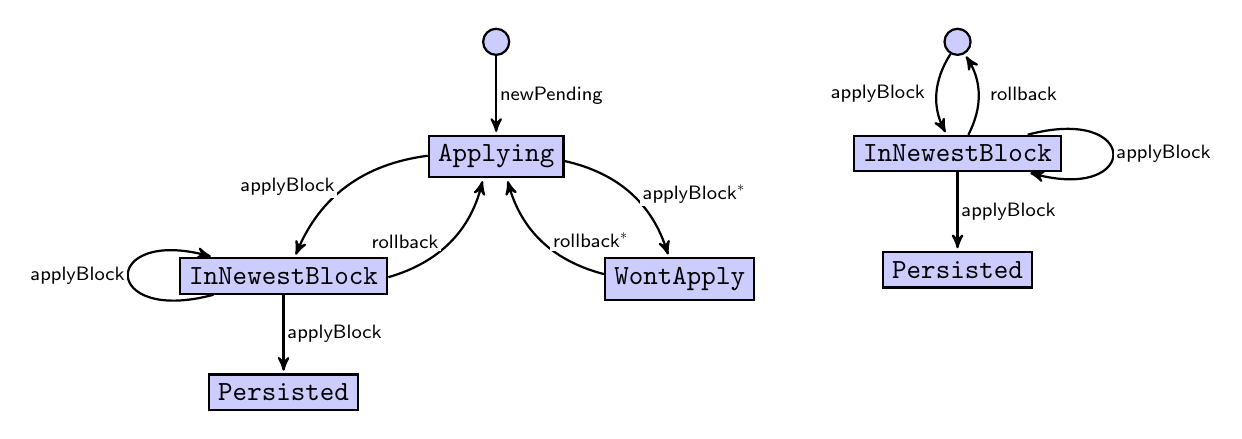
\begin{tikzpicture}[->,>=stealth',shorten >=1pt,auto,node distance=2cm,
  thick,main node/.style={rectangle,fill=blue!20,draw,minimum size=1mm}]

  \node[main node,style={circle}] (LStart) {};
  \node[main node] (LApplying)      [below=1cm of LStart] {\texttt{Applying}};
  \node[main node] (LInNewestBlock) [below left=1cm and 0.5cm of LApplying] {\texttt{InNewestBlock}};
  \node[main node] (LWontApply)     [below right=1cm and 0.5cm of LApplying] {\texttt{WontApply}};
  \node[main node] (LPersisted)     [below =1cm of LInNewestBlock] {\texttt{Persisted}};

  \path[every node/.style={font=\sffamily\scriptsize,
      fill=white,inner sep=1pt}]
    % Right-hand-side arrows rendered from top to bottom to
    % achieve proper rendering of labels over arrows.
    (LStart)
      edge node {$\mathsf{newPending}$} (LApplying)
    (LApplying)
      edge [bend right=30] node[left=1mm] {$\mathsf{applyBlock}$} (LInNewestBlock)
      edge [bend left=30]  node[right=1mm] {$\mathsf{applyBlock}^*$} (LWontApply)
    (LInNewestBlock)
      edge [loop left]     node {$\mathsf{applyBlock}$} (LInNewestBlock)
      edge [bend right=30] node[left=1mm] {$\mathsf{rollback}$} (LApplying)
      edge node {$\mathsf{applyBlock}$} (LPersisted)
    (LWontApply)
      edge [bend left=30] node[right=1mm] {$\mathsf{rollback}^*$} (LApplying)
    ;

  \node[main node,style={circle}] (RStart) [right=5.5cm of LStart] {};
  \node[main node] (RInNewestBlock) [below=1cm of RStart] {\texttt{InNewestBlock}};
  \node[main node] (RPersisted)     [below=1cm of RInNewestBlock] {\texttt{Persisted}};

  \path[every node/.style={font=\sffamily\scriptsize,
      fill=white,inner sep=1pt}]
    % Right-hand-side arrows rendered from top to bottom to
    % achieve proper rendering of labels over arrows.
    (RStart)
      edge [bend right=30] node[left=1mm] {$\mathsf{applyBlock}$} (RInNewestBlock)
    (RInNewestBlock)
      edge [loop right]     node {$\mathsf{applyBlock}$} (RInNewestBlock)
      edge [bend right=30] node[right=1mm] {$\mathsf{rollback}$} (RStart)
      edge node {$\mathsf{applyBlock}$} (RPersisted)
    ;
\end{tikzpicture}
\caption{\label{fig:transaction_state}Transaction state transitions (outgoing, \emph{left}, and incoming, \emph{right})}
\end{figure}

\section{Transaction Submission}
\label{sec:transaction_submission}

An actual implementation of the wallet needs to broadcast pending transactions
to the network, monitor when they get included in the blockchain, re-submit them
if they don't get included, and perhaps eventually decide to give up on them if
for some reason they do not get included.

This functionality does not need to be part of the wallet proper. In
\cref{sec:submission_interface} we will discuss the interface to this
component, and in \cref{sec:submission_implementation} we will give a
concrete simple implementation (which however still ignores any actual
networking issues).

\subsection{Interface}
\label{sec:submission_interface}

The interface to the transaction submission layer is shown in
\cref{fig:transaction_submission_layer}. It is of a similar nature as
interface to the wallet itself (\cref{fig:wallet_interface}). Just like
the wallet expects to be notified of events such as `new block arrived' and
`user submitted a new transaction', the submission layer expects to be notified
when the set of pending transactions grows or shrinks, and whenever a time slot
has passed (more on that below).

\begin{figure}
\begin{align*}
\mathsf{addPending} & :: \mathbb{P}(\mathsf{Tx}) \rightarrow \mathsf{Submission} \rightarrow \mathsf{Submission} \\
\mathsf{remPending} & :: \mathbb{P}(\mathsf{Tx}) \rightarrow \mathsf{Submission} \rightarrow \mathsf{Submission} \\
\mathsf{tick}       & :: \mathsf{Submission} \rightarrow (\mathbb{P}(\mathsf{Tx}), \mathsf{Submission})
\end{align*}
\caption{\label{fig:transaction_submission_layer}Transaction submission layer}
\end{figure}

It is the responsibility of the wallet to
%
\begin{itemize}
\item call $\mathsf{addPending}$ on $\mathsf{newPending}$ and (possibly) on $\mathsf{rollback}$
\item call $\mathsf{remPending}$ on $\mathsf{applyBlock}$ and $\mathsf{cancel}$
\end{itemize}

In addition there must be a thread that periodically calls $\mathsf{tick}$, to
give the submission layer a chance to resubmit transactions that haven't made it
into the blockchain yet. The set of transactions returned by $\mathsf{tick}$ are
the transactions that the submission layer gave up on (see below); the wallet
should remove such transactions from its $\mathit{pending}$ set. From the point
of view of the wallet model this corresponds to a new function
%
\begin{align*}
& \mathsf{cancel} :: \mathbb{P}(\mathsf{Tx}) \rightarrow \mathsf{Wallet} \rightarrow \mathsf{Wallet} \\
& \mathsf{cancel} ~ \mathit{txs} ~ (\mathit{checkpoints}, \mathit{txInfo}) = (\mathsf{map} ~ \mathsf{cancel'} ~ \mathit{checkpoints}, \mathit{txInfo}) \\
& \qquad \text{where} ~ \mathsf{cancel}' ~ (\mathit{utxo}, \mathit{pending}, \mathit{blockMeta}) = (\mathit{utxo}, \mathit{pending} \setminus \mathit{txs}, \mathit{blockMeta})
\end{align*}
%
By the logic of \cref{sec:transaction_status}, such a transaction would
be reported as $\mathtt{WontApply}$. Since we removed the transaction from the
$\mathit{pending}$ set in all checkpoints\footnote{If the overhead of traversing
all checkpoints is too large, an alternative implementation strategy would to be
maintain an explicit $\mathit{cancelled}$ set of transaction as part of the
wallet's state.}, however, a rollback won't reintroduce it into
$\mathit{pending}$; if the user wants to explicitly tell the wallet to try this
transaction again they will need to call $\mathsf{newPending}$. Effectively,
$\mathsf{cancel}$ becomes a secondary way in which a transaction may go from
$\texttt{Applying}$ to $\texttt{WontApply}$ (arrow $\mathsf{applyBlock}^*$), and
$\mathsf{newPending}$ a secondary way to get back from $\texttt{WontApply}$ to
$\texttt{Applying}$ (arrow $\mathsf{rollback}^*$).

\subsection{Implementation}
\label{sec:submission_implementation}

\cref{fig:submission_layer_impl} shows a simple implementation of the
submission layer.  Part of the goal of this section is to show that the
submission layer has sufficient information and does not need further support
from the core wallet layer---indeed, does not need to know it exists at all.

The state of the submission layer consists of a mirror copy of the pending set
of the wallet, as well as a schedule of which transactions to (re)submit next.
The schedule is modelled as a simple list of time slots, recording for each slot
the transactions that should be submitted, along with a submission count for
each transaction.
%
\begin{itemize}
\item When the submission layer is notified of new pending transactions,
it adds those to its $\mathit{pending}$ set and schedules them to be submitted
in the next slot, recording a initial submission count of 0.
\item When the wallet tells the submission layer that some transactions are
no longer pending (because they have been confirmed, because they have become
invalid, or for other reasons), the submission layer simply removes them
from its local $\mathit{pending}$ set.
\item The submission layer is parameterised over a `resubmission function'
$\varrho$. At the start of each time slot, the submission layer calls $\varrho$
to resubmit the set of transactions that are due, possibly dropping some
transactions that have reached a maximum submission count.
\end{itemize}

Although our model here does not deal with actual networking concerns, a
typical side-effectful implementation of $\varrho$ would
%
\begin{itemize}
\item Drop any transactions that have reached their maximum submission
count, possibly notifying the user
(note that $\varrho$ only gets called for transactions that are still listed as
pending).
\item Resubmit the remaining transactions to the network, and reschedule them
for the next attempt later. If desired, the submission count can be used to
implement exponential back-off.
\end{itemize}

The concept of time slots is essentially private to the submission layer; it
can, but does not have to, line up with the underlying blockchain slot length
(indeed, we don't need to assume that the underlying blockchain even \emph{has}
a slot length).

In principle $\mathit{pending}$ could be dropped from the submission layer; the
reason that we don't is that this would mean that $\mathsf{remPending}$ would
have to traverse the entire schedule to remove the transactions from each slot.
By keeping a separate $\mathit{pending}$ set we avoid this traversal, only
checking the pending set at the point where we need it. The wallet's
$\mathit{pending}$ set and the submission layer's one don't need to be in
perfect sync:
%
\begin{itemize}
\item If
\begin{math}
t \in    \mathit{pending}_\mathsf{Wallet} \text{ but }
t \notin \mathit{pending}_\mathsf{Submission}
\end{math}
(yet), transaction $t$ will just be submitted a little bit later.

\item If
\begin{math}
t \notin \mathit{pending}_\mathsf{Wallet} \text{ but (still) }
t \in    \mathit{pending}_\mathsf{Submission}
\end{math}
then (depending on the submission count) the submission layer may resubmit a
transaction which has already been included in the blockchain, or report the
transaction as `dropped'. The former is harmless; the latter at worst simply
confusing. Moreover,  this may happen even if the wallet and the submission
layer \emph{are} synchronised: it's entirely possible that the transaction has
been included in the blockchain but the wallet hasn't been informed of the block
yet.
\end{itemize}

Although the specification uses a simple list for its schedule, if the overhead
of a linear scan over all time slots to reschedule transactions is unacceptable,
it can of course easily use a different list-like datatype such as a
fingertree\footnote{Available in Haskell as \texttt{Data.Sequence}.}
\citep{hinze_paterson_2006}.

\begin{figure}
%
\emph{Types}
%
\begin{align*}
  \mathit{schedule}
& \in \mathsf{Schedule} = [\mathsf{Tx} \mapsto \mathbb{N}]
\end{align*}
%
\emph{Parameters}
%
\begin{align*}
  \varrho
& \in (\mathsf{Tx} \mapsto \mathbb{N}) \times \mathsf{Schedule} \rightarrow \mathbb{P}(\mathsf{Tx}) \times \mathsf{Schedule} & \text{Resubmission}
\end{align*}
%
\emph{State}
%
\begin{align*}
  (\mathit{pending}, \mathit{schedule})
& \in \mathsf{Submission} = \mathsf{Pending} \times \mathsf{Schedule}
\end{align*}
%
\emph{Atomic updates}
%
\begin{align*}
  \mathsf{addPending}
    ~ \mathit{txs}
    ~ (\mathit{pending}, \mathit{schedule})
& = ( \mathit{pending} \cup \mathit{txs}
    , \{ \mathit{tx} \mapsto 0 \mid \mathit{tx} \in \mathit{txs} \} : \mathit{schedule}
    )
\\
  \mathsf{remPending}
    ~ \mathit{txs}
    ~ (\mathit{pending}, \mathit{schedule})
& = ( \mathit{pending} \setminus \mathit{txs}
    , \mathit{schedule}
    )
\end{align*}
\begin{align*}
& \mathsf{tick} ~ (\mathit{pending}, []) = (\emptyset, (\mathit{pending}, [])) \\
& \mathsf{tick} ~ (\mathit{pending}, \mathit{due} : \mathit{schedule})
= (\mathit{dropped}, (\mathit{pending}, \mathit{schedule'})) \\
& \qquad\text{where~} (\mathit{dropped}, \mathit{schedule}')
= \rho(\mathit{pending} \restrictdom \mathit{due}, \mathit{schedule})
\end{align*}
%
\caption{\label{fig:submission_layer_impl}Submission layer implementation}
\end{figure}

\subsection{Persistence}

The state of the submission layer does not need to be persisted. If the wallet
is shutdown for some period of time, the submission layer can simply be
re-initialised from the state of the wallet, starting the submission process
afresh for any transactions that the wallet still reports as pending. As long
as the submission layer is able to report `time until dropped' for still
pending transactions, so that the user can see that all pending transactions
have been reset to the initial expiry time of say 1 hour, it will be clear to
the user what happened. This should be sufficient even for exchange nodes
(especially since they will shutdown the wallet only very rarely).

If this reset to 1 hour (or whatever the expiry time is) is not acceptable,
then the state of the submission layer \emph{does} need to be persisted.
The creation time of the transactions cannot be used, since this is a static
value and will not change when the transaction gets explicitly resubmitted
by the user after the submission layer decided to drop it.

\subsection{Transactions with TTL}
\label{sec:TTL}

Dropping transactions after a certain time has passed is merely a stop-gap
measure. Once a transaction has been broadcast across the network, it may be
included at any point, possibly long after the submission layer has given up on
it (unless the chain includes confirmed transactions that spends one or more of
the transaction's inputs).

The proper solution to this problem is to introduce a time-to-live (TTL) value
for transactions, stating that the transaction must be included in the
blockchain before a certain slot and simply dropped otherwise. A proper treatment
of TTL would require revisiting every aspect of this specification; for now
we just make a few observations:

\begin{itemize}
\item Once a TTL has been introduced, the core wallet \emph{itself} can remove
transactions from its $\mathit{pending}$ set once the TTL has expired.
\item This means that the submission layer does not need to implement expiry
anymore, although it may still wish to keep track of a submission count so that
it can implement exponential back-off.
\item Persistence for the submission layer becomes even less important.
The expiry of a transaction is now determined by the state of the blockchain,
and moreover once a transaction \emph{is} expired it cannot be resubmitted again
(a new transaction, with a new TTL, must be signed).
\end{itemize}

\section{Input selection}
\label{sec:input_selection}

In this wallet specification we assume that new transactions to be submitted are
provided to $\mathsf{newPending}$ fully formed. In reality this is preceded by a
process known as \emph{input selection} which, given a set of desired outputs
(that is, a \emph{payment} that the user wishes to make), selects one or more
inputs from the wallet's UTxO to cover that payment and the transaction fee,
returning any change back to the wallet. The result of input selection is a
fully formed transaction which can then be passed to $\mathsf{newPending}$. This
is summarised more formally in \cref{fig:input_selection_sig}.

\begin{figure}
\begin{align*}
& \mathsf{selectInputs} \in \mathsf{UTxO} \to \mathbb{P}(\mathsf{TxOut}) \to \mathsf{Maybe} ~ \mathsf{Tx} \\
\\
& \mathsf{Just} ~ (\mathit{inputs}, \mathit{outputs}') = \mathsf{selectInputs} ~ \mathit{utxo} ~ \mathit{outputs} \\
& \qquad \mathbf{ensures~}
\begin{array}[t]{l@{\;}l@{\;}l}
\mathit{inputs}          & \subseteq & \dom \mathit{utxo} \\
\range \mathit{outputs}' & \supseteq & \mathit{outputs}   \\
\multicolumn{3}{l}{\range \mathit{outputs}' \setminus \mathit{outputs} \subseteq \mathsf{TxOut_{ours}}} \\
\end{array}
\end{align*}
\caption{\label{fig:input_selection_sig}Specification of input selection}
\end{figure}

Input selection is a large topic which merits a detailed study in its own right.
Moreover, since input selection has multiple mutually incompatible goals, there
is no single one-size-fits-all input selection algorithm.  We will therefore
defer a detailed and formal discussion of input selection to a separate study.
Here we will merely list of of the goals of input selection, and list some
properties that a good input selection algorithm will have. We will also
briefly consider what kind of data structure can be used to make sure that
the asymptotic complexity of input selection is acceptable.

\subsection{Goals}

In this section we list some goals that a particular input selection algorithm
may have. As is well-known \citep{lopp:challenges}, many of these goals compete
with each other; it will therefore be important that wallet users can influence
this process, prioritising some goals over others.

\emph{Low transaction fees.}
Transactions must include a transaction fee, which is based on the size of the
transaction (\cref{app:transaction_fees}). A good input selection
algorithm will attempt to keep these transaction fees low. One complication here
is that the fee depends on the size of the transaction, but the size of
the transaction may depend on the fee since we may need to add more inputs to
the transaction in order to cover the fee. Thus fee calculation and input
selection are interdependent. There are situations where it is not immediately
obvious that there is a terminating algorithm for selecting inputs and fees
optimally. Note that minimising transaction fees over time does not necessarily
mean that every individual transaction will be as small as possible.

\emph{Cryptographic security.}
Once an input at an address has been spent, its public key is publicly
known and is arguably no longer suitable for very long term storage of funds due
to the evolution of cryptography. The standard solution with input selection is
to add a constraint that if we pick one input then we must pick all other inputs
that were output to the same address. This results in no more funds remaining at
the address (assuming an address non-reuse strategy such that there are no later
payments to that address).

\emph{Privacy.}
The privacy goal is to make it impractical for other people observing the
transactions in the ledger to tie an identity to all the funds belonging to that
identity. For instance, it is preferable to have a transactions with single
inputs only, since otherwise attackers can reasonably assume\footnote{In systems
such as Bitcoin there are services known as ``laundry services'', ``mixers'' or
``tumblers'' \citep{10.1007/978-3-319-70290-2_18}, which are trusted third
parties that combine payments from various users into a single transaction, to
break this assumption.}  that of all the transactions inputs belong to the same
identity \citep{fergal}. On the output side, we may wish to take steps to ensure
that attackers cannot easily identity which output is the change output
\citep{8260674}. For instance, for single payment transactions, we could try to
ensure that the change output is roughly as large as the payment itself. Some
systems give users the ability to override input selection on a per-transaction
bases (sometimes known as ``coin control''), since some transactions are more
sensitive than others.

\emph{UTxO size.}
A transaction with a single input and two outputs will increase the size of the
global UTxO by one entry, and (provided one of those is a change address), leave
the size of the wallet's own UTxO unchanged; since incoming transactions will
always grow the size of the wallet's UTxO, this means with such transactions the
size of the wallet's UTxO will also grow without bound over time. Since the UTxO
is kept in memory, this is undesirable. Instead input selection should attempt
to keep the size of the UTxO steady. More specifically, if incoming transactions
grow the wallet's UTxO by $n$ entries on average, and the ratio of incoming
transactions to outgoing transactions is $r : 1$, then ideally outgoing
transactions should shrink the wallet's UTxO by $r \times n$ entries on average.

\emph{Distribution of magnitude of unspent outputs.}
Input selection can try to keep the distribution of the magnitude of unspent
outputs close some ideal distribution. An obvious example is to avoid ``dust'':
many tiny unspent outputs that result from change outputs. More generally,
input selection can be given an ideal distribution a priori, or keep one
dynamically based on the payment requests that come in. An example of an
a-priori known requirement would be the ability to make payments of a certain
size; if the UTxO only contains small unspent outputs, then for very large
payments the resulting transaction might exceed the maximum transaction size.
Conversely, if the UTxO only contains large outputs, the wallet may be forced to
rely on unconfirmed transactions to maintain throughput, something we've
expressly disallowed in this specification (\cref{sec:updatePending})
because it has negative consequences on networking performance.
The privacy consequences of this kind of UTxO maintenance are far from obvious,
but we note that some authors claim it may actually \emph{help}
\citep[Section 2]{10.1007/978-3-642-39884-1_2}.

\subsection{Use cases}
\label{sec:input_selection_use_cases}

As an example of how different users might prioritise different goals,
we will consider two use cases, at opposite ends of the spectrum: small end
users and exchange nodes.

\emph{Exchange nodes.}
Exchanges have high rates of incoming and outgoing transactions, large overall
balances and will tend to have large UTxOs. For this use case we are concerned
with asymptotic complexity (due to the large UTxO) and have a goal of high
throughput, but we are not overly concerned with the goals of achieving privacy
or minimising fees. Exchanges tend to follow deposit policies which are
incompatible with the cryptographic security goal as described above, so this is
not a goal of the policy. Exchanges may occasionally need to make very large
payments.

\emph{Individual users.}
For individual users we assume a low rate of incoming and outgoing transactions
and a comparatively small UTxO. For this use case we are not too concerned with
asymptotic complexity as the UTxO is assumed to be small, nor with a goal of
high throughput. We are concerned with the privacy goal, as individual users
are able to use their wallets in a way that preserves a degree of privacy. We
are somewhat concerned with keeping fees reasonably low. Users may want the
ability to `empty their wallet' (i.e., create a single transaction that
spends all of the wallet's UTxO, sending it to a single output address.)

\subsection{Implementation notes}

A key operation required by input selection, independent of the specific policy,
will be to choose inputs from the UTxO of (roughly) a certain size. The easiest
way to do this is to keep the UTxO sorted by size, so that we can do binary
search for outputs within a certain range in $\order{n \log n}$ time. When an
unspent of a certain size is not available, there are two choices:
%
\begin{itemize}
\item Use a larger unspent output. The larger the unspent output we choose,
the larger the change value, endangering privacy concerns.
\item Use multiple smaller unspent outputs. This allows us to be more
accurate, but will lead to larger transactions and hence larger transaction
fees. In the extreme case the entire UTxO contains only small unspent outputs,
and we need to do a linear sweep over the UTxO to construct the transaction.
\end{itemize}
%
This is thus a tradeoff between privacy on the one hand and transaction size
and performance on the other.

Transaction fees can be (closely) approximated based on only the number of
inputs and outputs. Assuming that the UTxO has sufficiently many outputs
available that we do not need any of the fallback strategies, the number of
inputs and outputs is determined by the number of payments that the transactions
need to make, the privacy policy, and the UTxO maintenance policy. We can
therefore guess the transaction fee up-front, make sure to include it when we
select input amounts, and once we construct the final transaction shift any
excess into the change address(es).  If we do end up having to use the fallback
strategies, we will need to iterate this process (indeed, the added fee itself
might \emph{trigger} the need for a fallback).

\appendix

\section{Appendix: Transaction fees}
\label{app:transaction_fees}

Since this specification is not concerned with blockchain validation, it does
not require a formal treatment of transaction fees. Even new transactions
submitted to $\mathsf{newPending}$ are assumed to be fully formed and valid.
Indeed, the only section where we even need the concept of fees is
\cref{sec:input_selection} on input selection, where we mention that a
transaction constructed by input selection must satisfy the minimum fee
requirement. For completeness sake, in this appendix we outline how a
transaction fee is represented in Cardano, and how the minimum fee is computed.

Although our formalisation of UTxO style accounting is based on that of
\cite{utxo_accounting}, we diverge slightly from that formalisation and do
not represent fees explicitly. Instead, a transaction fee is simply the
difference between the transactions inputs and outputs:
%
\begin{align*}
& \mathsf{fee} \in \mathsf{UTxO} \to \mathsf{Tx} \to \mathsf{Coin} \\
& \mathsf{fee}_\mathit{utxo} ~ \mathit{tx} = \mathsf{totalin}_ \mathit{utxo} ~ \mathit{tx} - \mathsf{totalout} ~ \mathit{tx}
\end{align*}
%
where
%
\begin{IEEEeqnarray*}{LLLLL}
\mathsf{totalin}_\mathit{utxo} & ( & \mathit{inputs}, ~ \,\underline{\phantom{a}}\,  & ) & = \mathsf{balance} ~ (\mathit{inputs} \restrictdom \mathit{utxo}) \\
\mathsf{totalout}              & ( & \,\underline{\phantom{a}}\,, ~ \mathit{outputs} & ) & = \sum_{(\,\underline{\phantom{a}}\,, c) \in \mathit{outputs}} c
\end{IEEEeqnarray*}
%
where $\mathsf{totalin}$ is a function of the UTxO only because we need the UTxO
to know the size of a particular input (which, after all, is merely a
transaction hash and an index). It therefore has the precondition
%
\begin{align*}
& \mathsf{totalin}_\mathit{utxo} ~ (\mathit{inputs}, \,\underline{\phantom{a}}\,) \\
& \qquad \mathbf{requires~} \mathit{inputs} \subseteq \dom \mathit{utxo}
\end{align*}
%
This implicit representation of fees is suitable for this specification since we
don't need to reason about fees; moreover, this actually matches how fees are
represented in the actual Cardano blockchain (as well as in Bitcoin).

The minimum fee of a transaction is given by some linear function $f$ on the
serialised size of the transaction
%
\begin{align*}
\mathsf{minfee} & \in \mathsf{Tx} \to \mathsf{Coin} \\
\mathsf{minfee} & = f \circ \mathsf{size} \circ \mathsf{serialise}
\end{align*}

\bibliographystyle{apalike}
\bibliography{references}

\end{document}
